% setup
\documentclass[12pt,a4paper]{article}
%\documentclass[a4paper,12pt]{scrreprt}
\usepackage[left= 2.5cm,right = 2.5cm, bottom = 2.5 cm, top = 2.5cm, head = 14.5pt]{geometry}

\usepackage[utf8]{inputenc}
\usepackage[german]{babel}
\usepackage{csquotes}
\usepackage[T1]{fontenc}
\usepackage{amsmath}
\usepackage{amsfonts}
\usepackage{amssymb}

%matrices
\usepackage{blkarray}

%figures & images
\usepackage{graphicx}
\usepackage{subcaption}

%utils
\usepackage{color}
\usepackage{xcolor}
\usepackage{hyperref}
\usepackage{lipsum}

%Java und Javascript Code
\usepackage{listings}

%Abkürzugen
\usepackage[acronyms,automake,toc,nopostdot,nomain]{glossaries}
\makeglossaries
\loadglsentries{acronyms}

% Bibliographie
\usepackage[backend=biber,style=alphabetic,citestyle=authoryear]{biblatex}
\bibliography{Thesis}
\usepackage[nottoc]{tocbibind}

% Header Footer
\usepackage[automark,headsepline]{scrlayer-scrpage}
\clearpairofpagestyles
%\pagestyle{fancy}

\lehead{}
\chead{}
\ihead{\slshape}
%
\lefoot{}
\cfoot{}
\rofoot{\thepage}
\pagestyle{scrheadings}

% no indent
%\setlength{\parindent}{0pt}

% todo command
\newcommand\todo[1]{\textcolor{red}{#1}}

% Document Infos
\author{Amandus Stefan Butzer}
\title{Erstellung eines Routing-Profils für Feuerwehrfahrzeuge auf Basis von OpenStreetMap-Daten}
\date{\today}

\begin{document}
\begin{titlepage}
\begin{center}

	{\scshape\LARGE Ruprecht-Karls-Universität Heidelberg\par}
	\vspace{1.0cm}
	{\large Fakultät für Chemie und Geowissenschaften \par Geographisches Institut \par Abteilung Geoinformatik\par}
	\vspace{2.5cm}
	{\Huge\bfseries Erstellung eines Routing-Profils für Feuerwehrfahrzeuge auf Basis von OpenStreetMap-Daten\par}
	\vspace{2cm}
	{\Large\itshape Amandus Stefan Butzer\par}
	\vspace{2cm}
	{\LARGE\bfseries Bachelorarbeit\par}
	
	\vfill
	{\bfseries Geprüft von:}
	{\par 1. Prof. Dr. Alexander Zipf}
	{\par 2. Prof. Dr. Joao Porto de Albuquerque}

	\vfill

% Bottom of the page
	{\large \today\par}
\end{center}
\end{titlepage}

\newpage
\pagenumbering{Roman}

{\centering\section*{Zusammenfassung}}
\todo{Deutsche Kurzfassung}\par
\lipsum

\newpage
{\centering\section*{Abstract}}
\todo{Abstract in Englisch}
\lipsum

\newpage
\tableofcontents

\newpage
\listoffigures

%Abkürzungsverzeichnis
\printglossary[type=\acronymtype, title=Abkürzungsverzeichnis, toctitle=Abkürzungsverzeichnis]

\newpage
\pagenumbering{arabic}
\section{Einleitung}

\subsection{Motivation}
Zum Zeitpunkt der Erstellung dieser Arbeit ist der Verfasser in der Geoinformatik Abteilung des Geographischen Instituts der Ruprecht-Karls-Universität Heidelberg als wissenschaftliche Hilfskraft im Projekt \gls{ors} tätig. Dieser bietet neben einer Fülle von Webdiensten, wie Geocoding und Routing, auch einen Isochronen-Service an. Mit Isochronen werden Orte bestimmt, die von einem Standort aus in einer bestimmten Zeit erreicht werden können. Für Unternehmen ist so eine Analyse zum Beispiel bei der Standortwahl zur Berechnung von Umsatzpotentialen interessant. Arbeitnehmer können über Isochronen geeignete Wohnorte für eine zukünftige Arbeitsstelle ermitteln. Bus und Bahn richten an Isochronen ihre Verkehrsnetze aus oder legen Tarifzonen damit fest.
Für Polizei, Rettungsdienst sowie Feuerwehr geht es vor allem um das Einhalten amtlich vorgegebener zeitlicher Hilfsfristen. Diese stellen eine bedeutende Eigenschaft für die Planung und Qualität der Einsätze von Feuerwehr und Rettungsdienst dar.\par
Der Brandschutz ist im Gegensatz zum Rettungsdienst eine kommunale Aufgabe und unterliegt nur in manchen Bundesländern bestimmten Standards (\cite{bedarfsplan}). Daher bedienen sich diese Organisationen unterschiedlicher Hilfsmittel um Bedarfspläne für ihren Standort zu erstellen.
\medskip

Da mit dem Isochronen-Service jene zeitlichen Erreichbarkeitsanalysen durchgeführt werden können, ist dieser für die Erstellung eines Brandschutzbedarfsplans der Feuerwehr geeignet. Jedoch kann der Dienst in seiner bisherigen Form noch nicht alle erforderlichen Anforderungen für Einsatzfahrzeuge erfüllen. Um diese Nachteile zu überwinden, wurde eine Forschungskooperation mit der \gls{ffl} eingegangen.
\vspace{1.2cm}

\textbf{§35 Abs. 1 StVO:}
\begin{quotation}
\label{cit:STVO}
{\itshape\rmfamily ''Von den Vorschriften dieser Verordnung sind die Bundeswehr, die Bundespolizei, die Feuerwehr, der Katastrophenschutz, die Polizei und der Zolldienst befreit, soweit das zur Erfüllung hoheitlicher Aufgaben dringend geboten ist.''}
\end{quotation}

\vspace{1.2cm}

Dieser kurze Absatz der Straßenverkehrs-Ordnung ermöglicht Einsatzfahrzeugen sich unter Benutzung von Martinshorn und Blaulicht über jede Vorschrift im Straßenverkehr hinwegzusetzen. In einem Notfall hat das schnellste Erreichen des Zielorts eine höhere Priorität als Geschwindigkeitsbegrenzungen oder Fahrverbote. Bisher gibt es trotz einer großen Anzahl an Routing-Services keinen, der diese Tatsache berücksichtigt. 


\subsection{Zielsetzung}
Das Ziel dieser Arbeit ist in Kooperation mit der \gls{ffl} zu Ermitteln, bis zu welchem Grad diese Notstandsvollmachten im Ernstfall in Anspruch genommen werden können. Auf Basis dieser Informationen soll dann ein prototypisches Routing-Profil für Einsatzfahrzeuge entwickelt werden. Die Implementierung wird aufgrund des Umfangs einer Bachelorarbeit auf einen Fahrzeugtyp der Feuerwehr begrenzt. Dabei handelt es sich um Löschfahrzeuge der Klassen LF8, LF8/6 und MLF zwischen 3,5 und 7,5 Tonnen (je nach Beladung). Diese Typen wurden von der \gls{ffl} als erste Priorität empfohlen. Allerdings wird bei der Erstellung dieses Routing-Profils darauf geachtet, dass Erweiterungen für diverse Einsatzfahrzeuge einfach möglich sind.
\vspace{0.5cm}

Als Basis wird das Profil auf dem Backend\footnote{Programm und Datenbanken die sich zur Berechnung von Routen auf einem über das Internet ansprechbaren Server befinden} des bereits bestehenden Routing Service des \gls{ors} aufgebaut. Zusätzlich sollen Java Funktionen implementiert werden, die speziell auf das Emergency Profil zugeschnitten sind. Zur Darstellung wird das \gls{ors} Frontend\footnote{Graphische Benutzeroberfläche der \gls{ors}-Website mit der Anfragen an das Backend gestellt und die Antworten dargestellt werden können} mit Hilfe der Java-Script Programmiersprache angepasst. Dadurch können die Ergebnisse in verständlicher und anschaulicher Weise präsentiert werden.

\newpage
\section{Theoretische Grundlagen}

Als Grundlage für die Berechnung kürzester Wege in einem Straßennetzwerk wird die Graphentheorie als Teilgebiet der Mathematik herangezogen. 

\subsection{Graphentheorie}

Ein Graph ist eine abstrakte Struktur, die Objekte und deren Verbindungen untereinander modellieren kann. Die in der Graphentheorie verwendeten Termini belaufen sich dabei auf Ecken (engl: \textit{nodes} oder \textit{vertices}) für Objekte und Kanten (engl: \textit{edges}) für Verbindungen.
(\cite[49]{kurt})

Mathematisch ausgedrückt ist ein Graph ~$G$ die Funktion aus einer endlichen Eckenmenge ~$V$ und einer endlichen Kantenmenge ~$E$ (\cite[4]{theory})

	$$G = (V,E)$$

Für den Graphen in Abbildung ~\ref{simpleGraph} sehen ~$V$ und ~$E$ folgendermaßen aus:

$$V = \{(v_{1},v_{2},v_{3},v_{4},v_{5})\} $$
$$E = \{(v_{1}v_{2},v_{1}v_{3},v_{2}v_{3},v_{2}v_{3},v_{3}v_{5})\} $$

\begin{figure}[h]
\centering
\begin{subfigure}{0.49\textwidth}
\centering
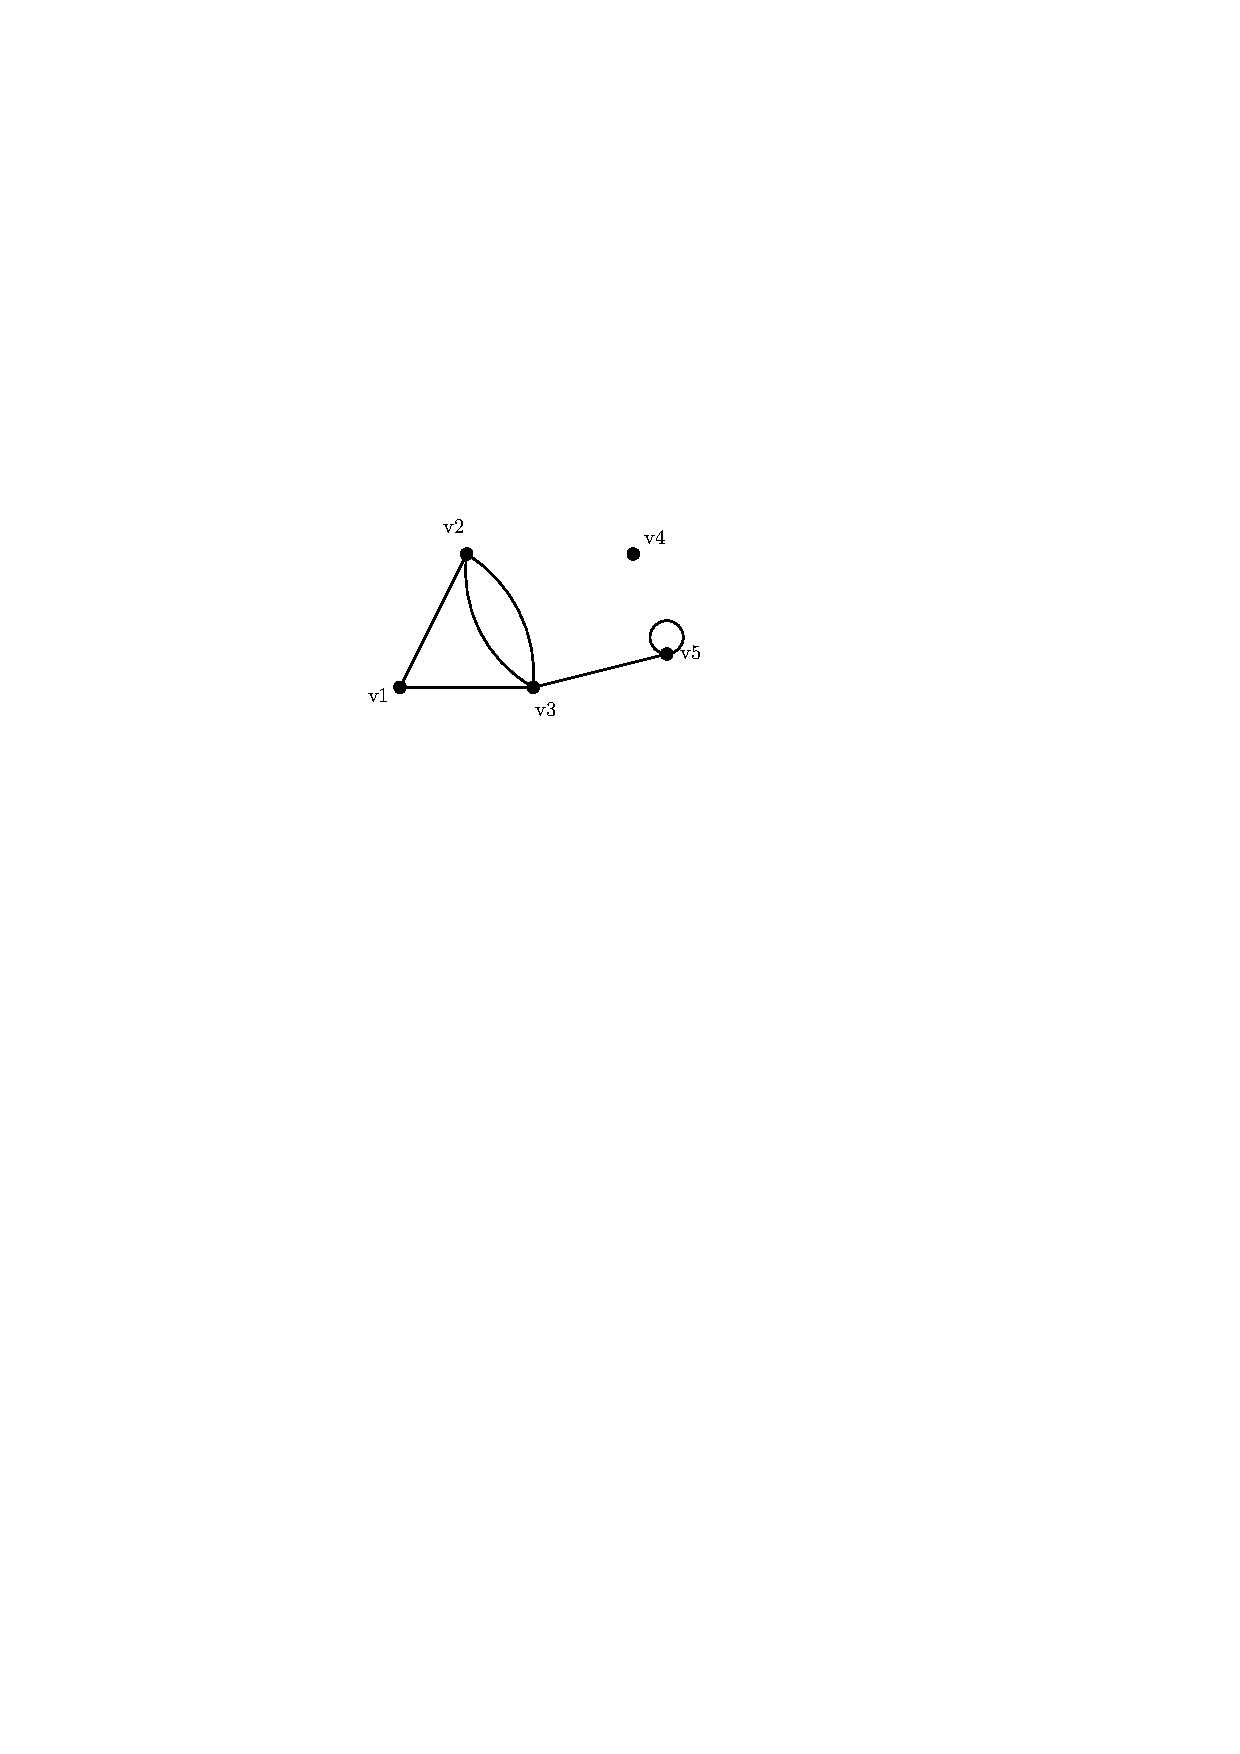
\includegraphics[width = \textwidth]{../media/simpel.pdf} \\
\caption{G}
\label{fig:simple}
\end{subfigure}
\begin{subfigure}{0.49\textwidth}
\centering
{
\begin{blockarray}{cccccc}
  & $v_{1}$ & $v_{2}$ & $v_{3}$ & $v_{4}$ & $v_{5}$ \\
\begin{block}{c(ccccc)}
  $v_{1}$ & 0 & 1 & 1 & 0 & 0 \\
  $v_{2}$ & 1 & 0 & 2 & 0 & 0 \\
  $v_{3}$ & 1 & 2 & 0 & 0 & 1 \\
  $v_{4}$ & 0 & 0 & 0 & 0 & 0 \\
  $v_{5}$ & 0 & 0 & 1 & 0 & 1 \\
\end{block}
\end{blockarray}
}
\vspace{0.1cm}
\caption{Adjazenzmatrix von G}
\label{mx:simple}
\end{subfigure}
\caption{Ein simpler Graph G}
\label{simpleGraph}
\end{figure}

Ein Vorteil von Graphen ist eine einfache Struktur. Dabei werden die Ecken als Punkte und die Kanten als Linien oder Pfeile dargestellt (Abbildung ~\ref{fig:simple}) (\cite[49]{kurt}). Zwischen zwei Ecken können einfache, mehrfache oder keine Kanten bestehen. Darüber hinaus können sie mit sich selbst verbunden sein und eine sogenannte Schlinge bilden ($v_{5}$). Sind zwei Ecken durch eine Kante verbunden bezeichnet man sie als \textit{adjazent}(benachbart). Ist eine Ecke der Start- oder Endpunkt einer Kante, werden beide Objekte als \textit{inzident} zueinander bezeichnet. Ist eine Ecke zu keiner Kante inzident heißt sie \textit{isoliert}. Ein Graph der keine isolierten Ecken besitzt heißt \textit{zusammenhängend}.(\cite[4\psq]{theory}) \par

Computer können Graphen sehr gut verarbeiten, da sich alle Ecken und Kanten in Form von Matrizen speichern lassen. Die Abbildung ~\ref{mx:simple} zeigt die Adjazenzmatrix des Graphen aus ~\ref{fig:simple}. Darin sind die Nachbarschaften für die jeweilige Eckenkombination gespeichert. Die Reihen sind die Start- und die Spalten die Endecken. Für eine existierende Kante wird eine ~$1$ und für keine Verbindung eine ~$0$ eingetragen. Die ~$2$ in Spalte $v_{2}$ und Reihe $v_{3}$ zeigt die Mehrfachkante zwischen den beiden Ecken an. Für ungerichtete Graphen ist eine Kante von $v_{1}$ nach $v_{2}$ äquivalent mit einer Kante von $v_{2}$ nach $v_{1}$. Daher ist die Adjazenzmatrix für ungerichtete Graphen spiegelsymmetrisch entlang der Hauptdiagonale ($v_{1}v_{1} \rightarrow v_{5}v_{5}$). Der Speicherbedarf für eine Matrix wird folglich halbiert, da die eine Hälfte mit der Anderen rekonstruiert werden kann (Abb.~\ref{mx:iso}). Besitzt der Graph keine Schlingen, besteht die Hauptdiagonale lediglich aus Nullen und kann ebenfalls eingespart werden (\cite[19]{algorithms}).

Im Folgenden werden nur zusammenhängende Graphen ohne Schlingen betrachtet, da diese für viele Problemstellungen irrelevant sind (\cite[4\psq]{theory}).

\begin{figure}[h]
\centering
\begin{subfigure}{0.42\textwidth}
\centering
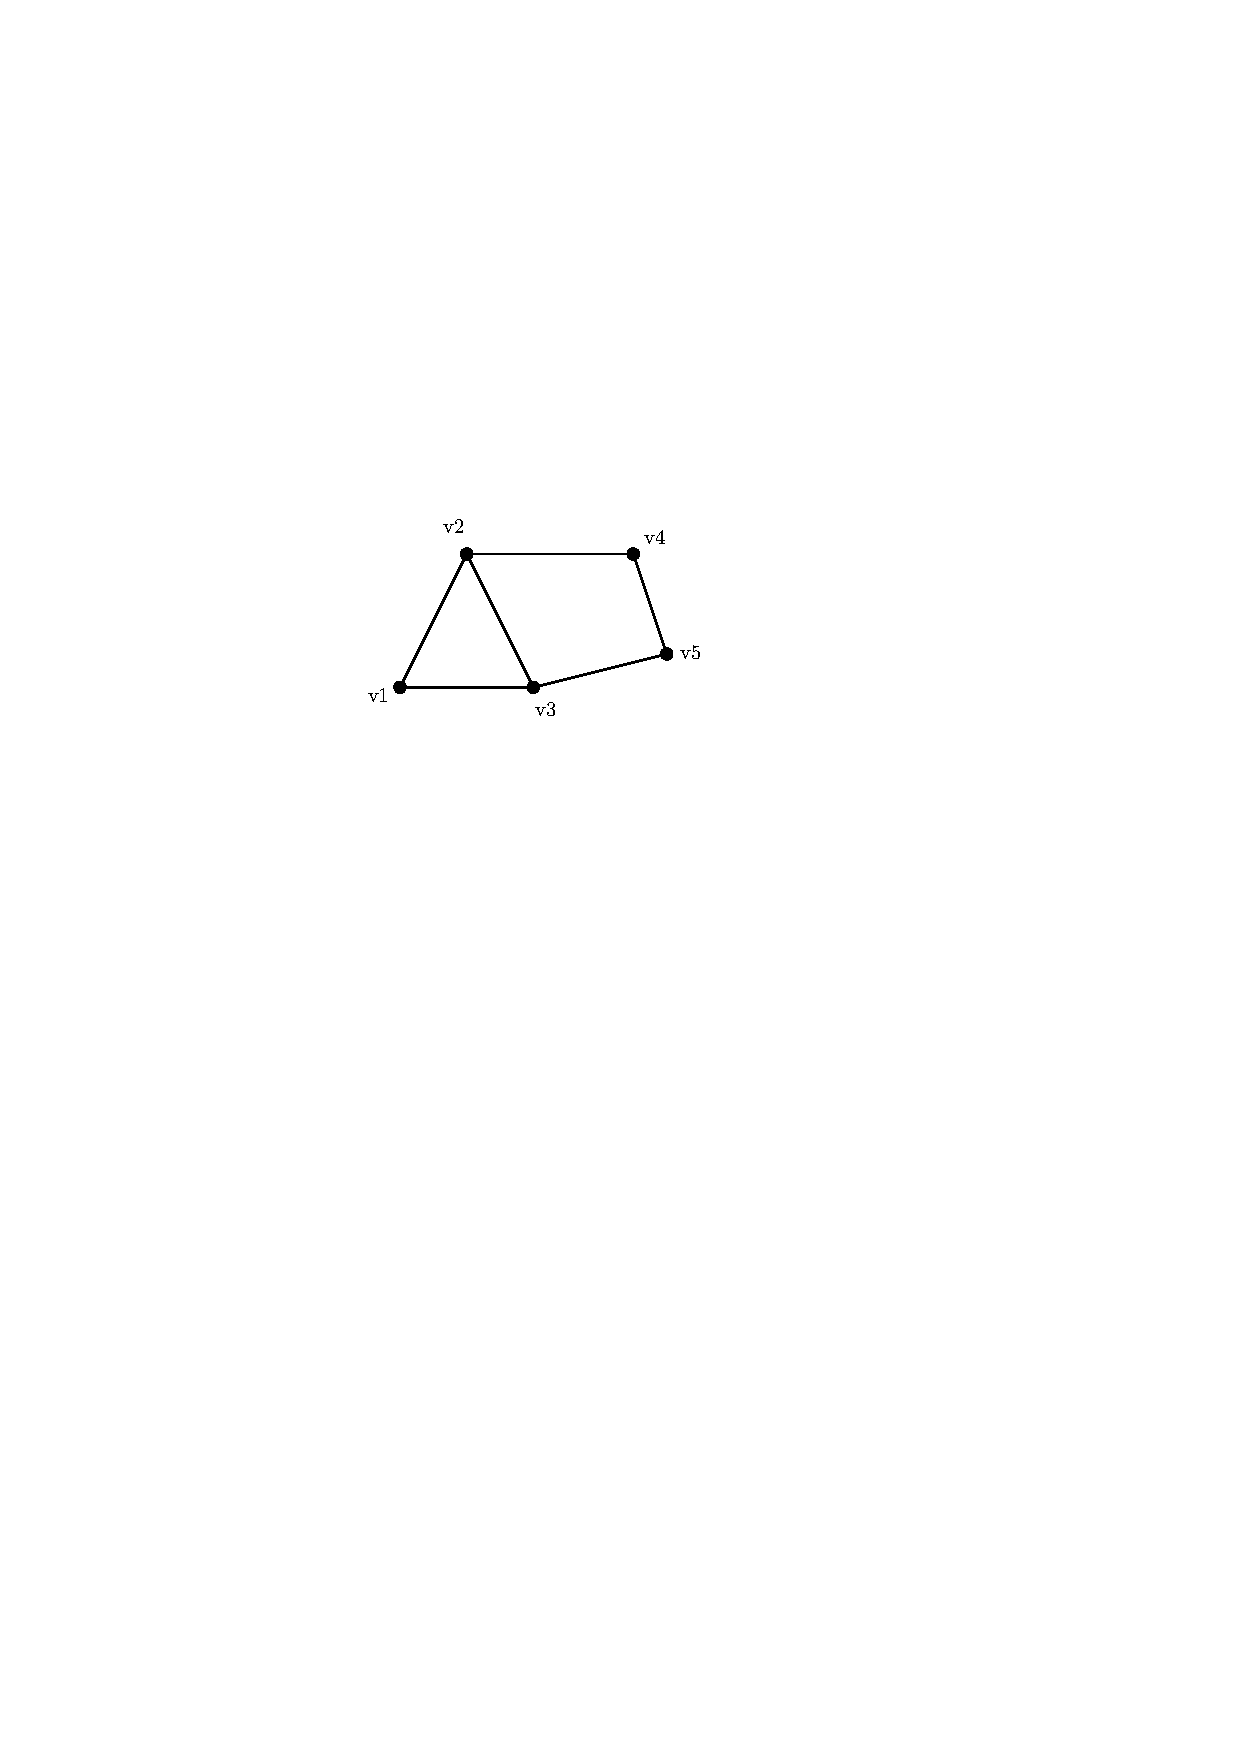
\includegraphics[width = \textwidth]{../media/iso1.pdf} \\
\caption{G}
\label{fig:iso1}
\end{subfigure}
\hspace{2cm}
\begin{subfigure}{0.30\textwidth}
\centering
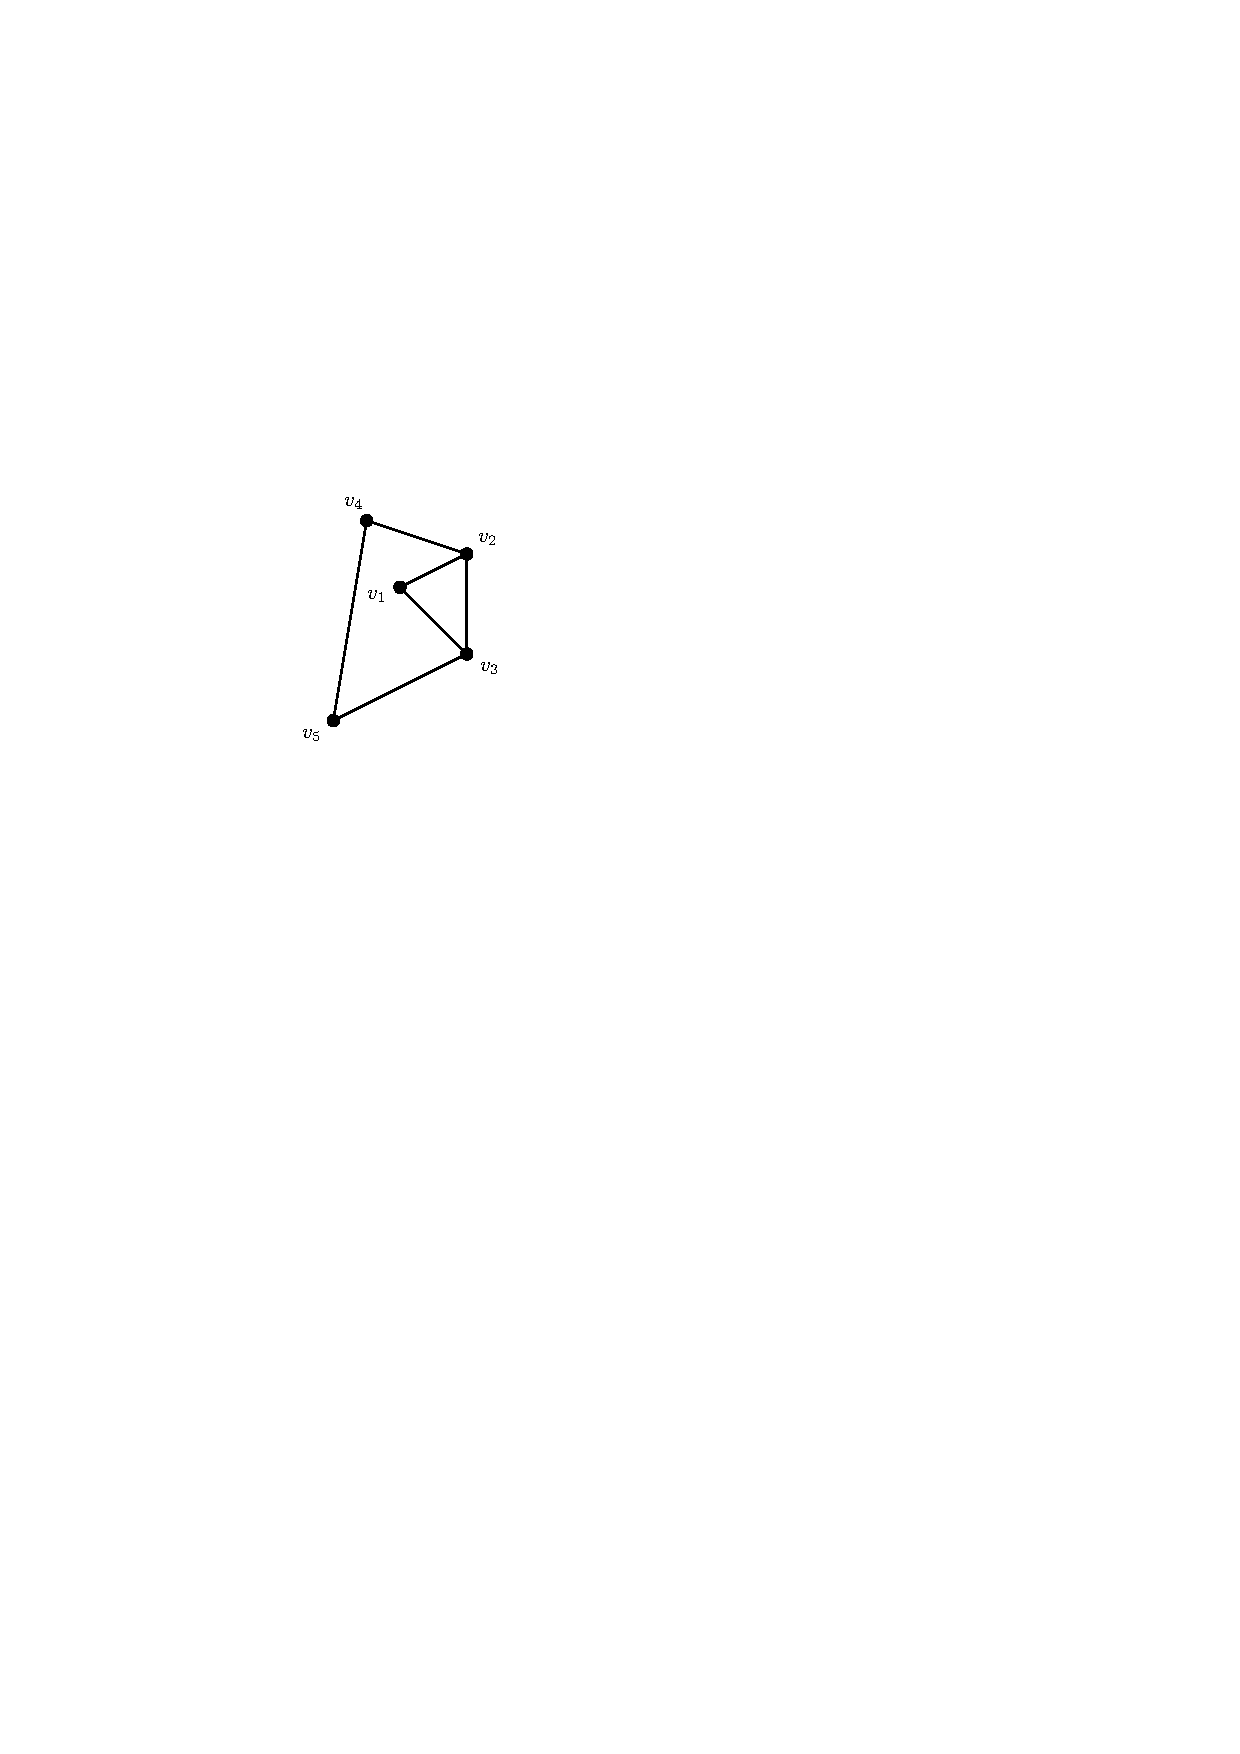
\includegraphics[width = \textwidth]{../media/iso2.pdf} \\
\caption{H}
\label{fig:iso2}
\end{subfigure}
\begin{subfigure}{0.40\textwidth}
\centering
\vspace{0.5cm}
{
\begin{blockarray}{cccccc}
  & $v_{1}$ & $v_{2}$ & $v_{3}$ & $v_{4}$ & $v_{5}$ \\
\begin{block}{c(ccccc)}
  $v_{1}$ & $\ddots$ & 1 & 1 & 0 & 0 \\
  $v_{2}$ &   & $\ddots$ & 1 & 1 & 0 \\
  $v_{3}$ &   &   & $\ddots$ & 0 & 1 \\
  $v_{4}$ &   &   &   & $\ddots$ & 1 \\
  $v_{5}$ &   &   &   &   & $\ddots$ \\
\end{block}
\end{blockarray}
}
\caption{Adjazenzmatrix von G und H}
\label{mx:iso}
\end{subfigure}
\caption{Zwei isomorphe Graphen G und H}
\label{isoGraph}
\end{figure}

Wenn zwei Graphen bei gleichbleibenden Nachbarschaften der Ecken aufeinander abgebildet werden können, spricht man von isomorphen Graphen (\cite[106]{theory}). Daraus ergibt sich für isomorphe Graphen auch immer eine gleiche Adjazenzmatrix (Abb.~\ref{isoGraph}).


\subsubsection{Gerichtete Graphen}
Im Gegensatz zu einem ungerichteten Graphen können bei einem gerichteten Graphen Kanten lediglich in einer Richtung durchlaufen werden. Die Kanten werden daher durch Pfeile anstatt Linien dargestellt. 

$$G = (V,R)$$

Demnach muss in Abbildung~\ref{fig:directed} um von $v_{5}$ nach $v_{4}$ zu gelangen der Weg über die Ecken $v_{3}$ und $v_{2}$ führen.

\begin{figure}[h]
\centering
\begin{subfigure}{0.49\textwidth}
\centering
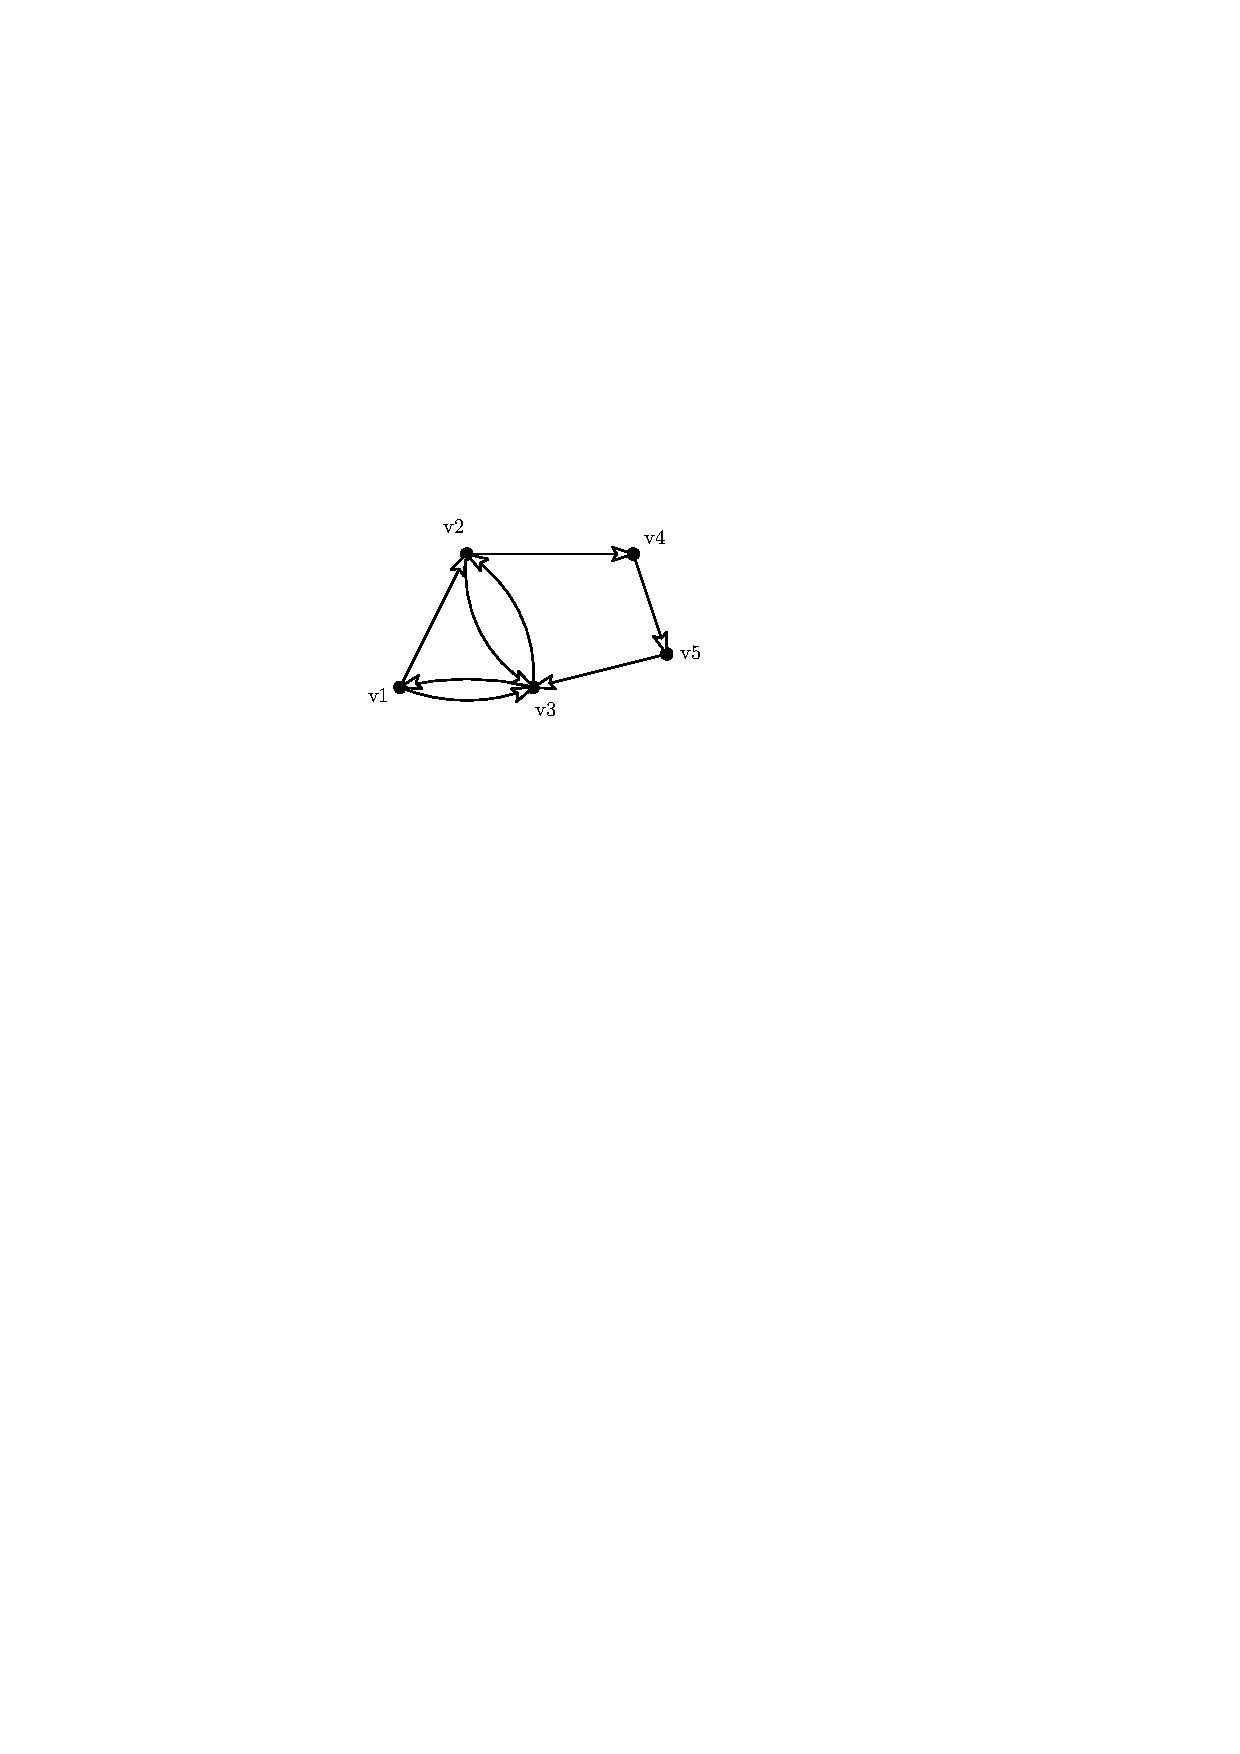
\includegraphics[width = \textwidth]{../media/gerichtet.pdf} \\
\caption{G}
\label{fig:directed}
\end{subfigure}
\begin{subfigure}{0.49\textwidth}
\centering
{
\begin{blockarray}{cccccc}
  & $v_{1}$ & $v_{2}$ & $v_{3}$ & $v_{4}$ & $v_{5}$ \\
\begin{block}{c(ccccc)}
  $v_{1}$ & 0 & 1 & 1 & 0 & 0 \\
  $v_{2}$ & 0 & 0 & 1 & 1 & 0 \\
  $v_{3}$ & 1 & 1 & 0 & 0 & 0 \\
  $v_{4}$ & 0 & 0 & 0 & 0 & 1 \\
  $v_{5}$ & 0 & 0 & 1 & 0 & 0 \\
\end{block}
\end{blockarray}
}
\vspace{0.1cm}
\caption{Adjazenzmatrix von G}
\label{mx:directed}
\end{subfigure}
\caption{Ein gerichteter Graph G}
\label{directedGraph}
\end{figure}

\subsubsection{Gewichtete Graphen}
In dieser Arbeit bezeichnet der Begriff \textit{gewichteter Graph} einen Kanten-gewichteten Graphen, bei dem jeder Kante ein Wert ~$c$ zugewiesen wird.

$$G = (V,E)$$ mit $$c: E \rightarrow \mathbb{R}$$

Neben dem Kanten-gewichteten gibt es auch Knoten-gewichtete Graphen, bei welchen entsprechend die Knoten gewichtet werden. Diese werden aber nur für wenige Problemstellungen benötigt und sind hier nicht von Belang. Gewichtete Graphen können gerichtet und ungerichtet sein. Ein klassisches Beispiel hierfür ist der Linien-Netzplan einer Straßenbahn, bei dem die Knotenpunkte einzelne Haltestellen darstellen und die Kantengewichte die benötigten Minuten beinhalten.

\begin{figure}[h]
\centering
\begin{subfigure}{0.49\textwidth}
\centering
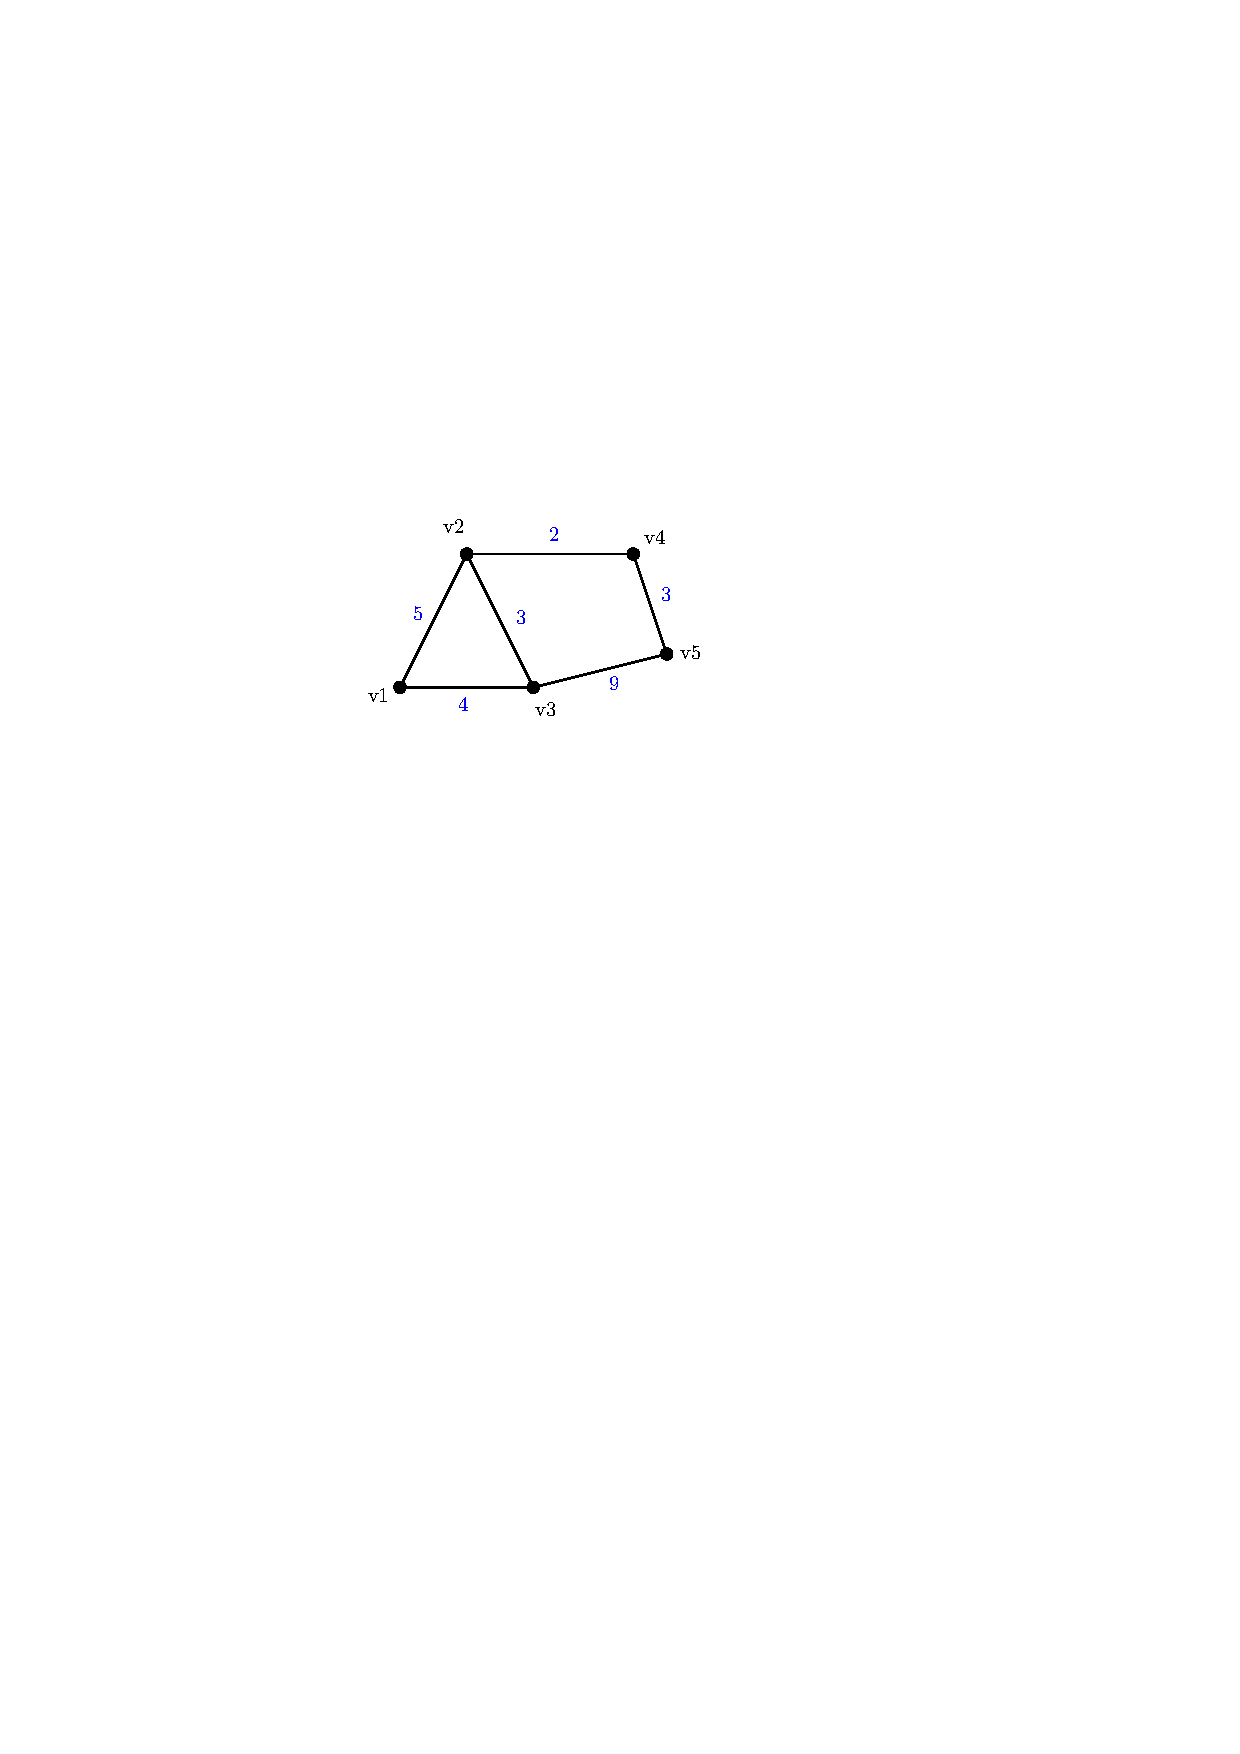
\includegraphics[width = \textwidth]{../media/gewichtet.pdf} \\
\caption{G}
\label{fig:weighted}
\end{subfigure}
\begin{subfigure}{0.49\textwidth}
\centering
{
\begin{blockarray}{cccccc}
  & $v_{1}$ & $v_{2}$ & $v_{3}$ & $v_{4}$ & $v_{5}$ \\
\begin{block}{c(ccccc)}
  $v_{1}$ & 0 & 5 & 4 & 0 & 0 \\
  $v_{2}$ & 5 & 0 & 3 & 2 & 0 \\
  $v_{3}$ & 4 & 3 & 0 & 0 & 9 \\
  $v_{4}$ & 0 & 2 & 0 & 0 & 3 \\
  $v_{5}$ & 0 & 0 & 9 & 3 & 0 \\
\end{block}
\end{blockarray}
}
\vspace{0.1cm}
\caption{Adjazenzmatrix von G}
\label{mx:weighted}
\end{subfigure}
\caption{Ein gewichteter Graph G}
\label{weightedGraph}
\end{figure}

Mit gewichteten Graphen können diverse Problemstellungen gelöst werden, zum Beispiel die Bestimmung maximaler (Durch-)Flüsse in Rohrsystemen oder das Berechnen kürzester Wege. Andererseits kann ein gewichteter Graph auch für Routing-Zwecke eingesetzt werden, indem räumliche Positionen sowie Eigenschaften von Straßen in der Datenstruktur eines Graphen gespeichert werden.

\subsubsection{Bau eines Graphen aus OpenStreetMap Daten}
\label{sec:osmgraph}

Die \gls{osm} Datenstruktur kann als Graph abgebildet werden. Hier werden Punktobjekte als \textit{Nodes}(Knoten) und Linienobjekte wie Straßen als \textit{Ways}(Wege) bezeichnet. Ein Way ist dabei die Verbindung zwischen zwei Nodes. Zusätzlich gibt es \textit{Relations}(Relationen) die einem Set aus Nodes und Ways einen funktionalen Zusammenhang zuschreiben. Für Straßennetze kann dies durchaus hilfreich sein um beispielsweise unterschiedliche Segmente eines Autobahnsegmentes zusammenzufassen oder um Abbiegebeschränkungen an Kreuzungen zu beschreiben (\cite{osmrelation}).

Um aus den \gls{osm} Daten einen routingfähigen Graphen zu erhalten, müssen zuerst alle benutzbaren Nodes und Ways extrahiert werden um sie dann anhand ihrer \gls{osm}-Tags zu identifizieren. Dazu gehören alle Arten von Straßen und Wegen sowie als befahrbar gekennzeichneten Ways (zum Beispiel asphaltiert, allerdings ohne Straßentyp). Für das Routing sind vor allem Verbindungspunkte wie Kreuzungen, Ab- und Auffahrten etc. sowie Sackgassen interessant. Daher werden diese \textit{Tower Nodes} aus den importierten Daten ermittelt. Anschließend werden die Straßen anhand der Verbindungspunkte segmentiert. Danach werden die Verbindungen zwischen den Tower Nodes berechnet und anhand der Distanz gewichtet. Das Grundgerüst des eigentlichen Routing-Graphen ist damit erstellt. Einbahnstraßen und Abbiegebeschränkungen werden berücksichtigt und geben die Richtung der Edges an (\cite{osmgraph}). Die Punkte zwischen zwei Tower Nodes werden \textit{Pillar Nodes} genannt. Sie werden als \textit{WayGeometry} auf der jeweiligen Edge gespeichert, da sie nicht für den Routing Vorgang benötigt werden (Abbildung ~\ref{fig:tower}). Das Routing ist dadurch um ungefähr das 8-fache schneller (\cite{graphhopper}). Relevante Attribute wie Geschwindigkeit oder Straßentyp werden vereinheitlicht und als \textit{Flags} (Markierung)auf der Edge gespeichert. Diese sind für die individuelle Gewichtung bei der Routenfindung interessant. (Mehr zu Gewichtung später in Kapitel ~\ref{backendGraphBuild}(\todo{stimmt die reihenfolge max?}). Zuletzt wird der Graph abgespeichert und ist für Routing Abfragen bereit (\cite{osmgraph}). 

\begin{figure}[h]
\centering
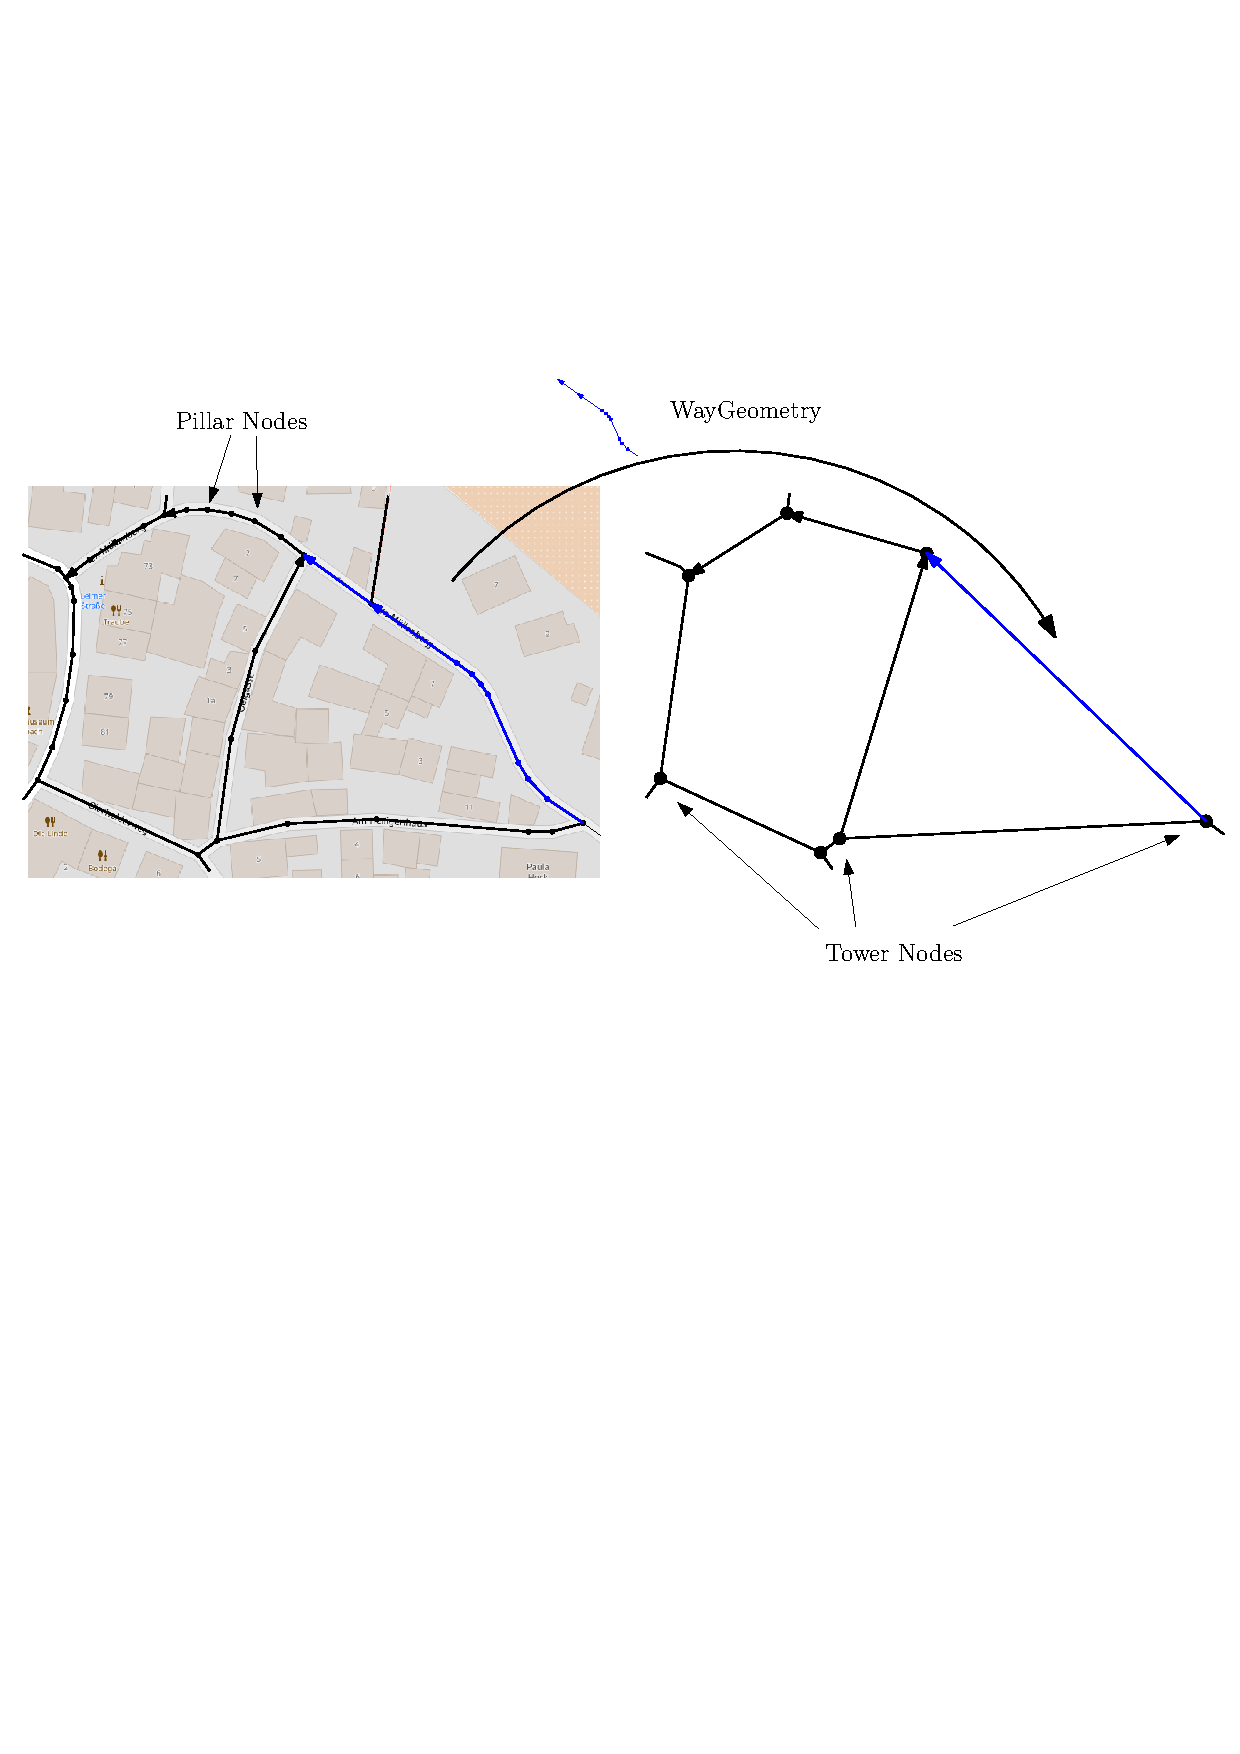
\includegraphics[width = \textwidth]{../media/towers.pdf} \\
\caption{Simplifizierung eines OSM Datensatzes}
\label{fig:tower}
\end{figure}

\subsection{Routing}

Routing bezeichnet den Vorgang in einem Netzwerk Wege zu finden, auf denen Datenpakete entlang gesendet werden können. Diese Definition bezieht sich vor allem auf elektronische Datennetzwerke wie das Telefonnetz oder das Internet. Im Fachbereich der \gls{gis} werden hauptsächlich Straßennetze für Routing-Analysen verwendet (\cite[165]{handbook}). Ein Weg \textit{P} (\textit{engl: path}) von einem Startecke ~$s$ zu einem Zielecke ~$z$ ist eine Folge von benachbarten Ecken mit $s~$ als erster Ecke und $z~$ als letzter Ecke der Folge (\todo{Abb}).
Die Weglänge entspricht in einem gewichteten Graphen der Summe aller Kantengewichte.

Eine der wichtigsten Netzwerk-Analyse-Operationen ist die Berechnung des kürzesten Weges zwischen zwei Knoten. Jedes Navigationssystem muss diese Aufgabe erfüllen können. Ein kürzester Weg hat demnach die Eigenschaft, dass die Summe aller Kantengewichte, in anderen Worten die Kosten des Weges, minimal gegenüber allen anderen Wegen im Graphen ist.

\subsubsection{Shortest Path Problem}
Die nächstliegendste zu beleuchtende Problemstellung ist das \textit{Shortest Path Problem} welches aber nicht mit dem \textit{\gls{tsp}} verwechselt werden sollte. Beim \gls{tsp} ist die kürzeste Tour auf einem Graphen $G  = (V,E) = K_{n}$\footnote{$K_{n}$ bezeichnet einen vollständigen Graphen bei dem jede Ecke aus V mit jeder anderen Ecke verbunden ist} mit der Gewichtsfunktion $c: E \rightarrow \mathbb{R}_{+}$ gesucht, die jeden Knoten des Graphen besucht(\cite[135]{algorithms}).
Das Shortest Path Problem lässt sich in drei Typen untergliedern denen jeweils ein gerichteter Graph $G = (V,E)$ mit der Gewichtsfunktion $c: E \rightarrow \mathbb{R}$ zugrunde liegt. Beim \textit{\gls{spp}} wird der kürzeste Weg von einer Ecke $a~$ zu einer anderen Ecke $b~$ mit $a,b\in V$ gesucht. Das \textit{\gls{ssp}} möchte den kürzesten Weg einer Ecke $a~$ zu jeder anderen Ecke ermitteln (Formel ?). Das \textit{\gls{apsp}} sucht den kürzesten Weg von jeder Ecke zu jeder anderen Ecke in $V~$ (\cite[169\psq]{algorithms}).

Für eine Route von Startecke $s~$ zur Zielecke $z~$ ist das \gls{spp} demnach die richtige Wahl. Allerdings wird dazu das \gls{ssp} herangezogen, welches mit dem Algorithmus von Dijkstra gelöst werden kann.


\subsubsection{Dijkstra-Algorithmus}
\label{sec:dijkstra}
Der in 1959 von Edsger W. Dijkstra entwickelte Algorithmus (\cite{dijkstra}) benötigt einen gewichteten Graphen ohne negative Kantengewichte\footnote{Das Problem bei Graphen mit negativer Gewichtung entsteht, wenn diese auf einer Schlinge oder der Kante eines Rings liegen. Sobald der Algorithmus den Zyklus erreicht, werden die Kosten für die Ecken des Zyklus immer geringer. Die Kosten für den kürzesten Weg nähern sich $-\infty $ während der Algorithmus in einer endlos Schleife läuft. Deswegen ist der Dijkstra nur für positive Kantengewichte anwendbar (\cite[194\psq]{kurt})} sowie eine Startecke $s \in V$. Es gibt eine Warteliste $W_{s}$ mit unmarkierten \textit{gesichteten} Ecken. Dort sind für alle $v~$ die Kosten für den bisher kürzesten Weg von $s~$ und die jeweilige vorangehende Ecke auf diesem Weg gepeichert. Die Kosten können sich noch ändern wenn ein noch kürzerer Weg gefunden wird. Diese Liste enthält zu Beginn nur den Startpunkt $s~$ mit den trivialen Kosten $0~$. Es gibt eine weitere Liste der endgültig kürzesten Wege $K_{s}$ in der alle markierten Ecken gespeichert werden.

Dijkstra's Algorithmus markiert die Ecke mit den geringsten Kosten aus $W_{s}$ und verschiebt diese nach $K_{s}$. Nun werden alle benachbarten Ecken gesichtet und die Kosten berechnet. Die Kosten und der Vorgänger werden in $W_{s}$ gespeichert. Die Ecke mit den geringsten Kosten wird als nächstes markiert, da der Weg dorthin auf jeden Fall ein kürzester ist. Dieser Vorgang wird wiederholt bis alle Ecken aus $W_{s}$ markiert wurden und $W_{s}$ somit leer ist.

% Init Dijkstra
\begin{figure}[h]
\centering
\begin{subfigure}{0.49\textwidth}
\centering

\includegraphics[width = \textwidth]{../media/dijkstra.pdf} \\
\caption{G}
\label{fig:dijkstra}
\end{subfigure}
\begin{subfigure}{0.49\textwidth}
\centering
{
\begin{blockarray}{cccccc}
  & $v_{1}$ & $v_{2}$ & $v_{3}$ & $v_{4}$ & $v_{5}$ \\
\begin{block}{c(ccccc)}
  $v_{1}$ & 0 & 5 & 4 & 0 & 0 \\
  $v_{2}$ & 7 & 0 & 0 & 3 & 0 \\
  $v_{3}$ & 4 & 2 & 0 & 0 & 8 \\
  $v_{4}$ & 0 & 3 & 6 & 0 & 1 \\
  $v_{5}$ & 0 & 0 & 8 & 1 & 0 \\
\end{block}
\end{blockarray}
}
\vspace{0.1cm}
\caption{Adjazenzmatrix von G}
\label{mx:dijkstra}
\end{subfigure}
\caption{Ein gewichteter und gerichteter Graph G}
\label{dijkstraGraph}
\end{figure}

Die Funktionsweise des Dijkstra Algorithmus wird am Graphen aus Abbildung ~\ref{dijkstraGraph} mit der Startecke $s=v_{1}$ veranschaulicht.

Die erste Ecke der Warteschlange ist $s=v_{1}$. Da $s~$ der einzige Eintrag ist, sind die Kosten automatisch am geringsten. $s~$ wird von $W_{s}$ nach $K_{s}$ verschoben, markiert und die erreichbaren Ecken gesichtet. Das sind $v_{2}$ mit den Kosten $5~$ und $v_{3}$ mit den Kosten $4~$. Beide werden mit $v_{1}$ als Vorgänger in $W_{s}$ eingetragen.
Im zweiten Durchgang wird $v_{3}$ (geringste Kosten in $W_{s}$) markiert und nach $K_{s}$ verschoben. Über $v_{3}$ erreichbare Ecken sind $v_{5}$ mit $4+8=12$ Kosten und $v_{2}$ mit $4+2=6$ Kosten. Da bereits ein kürzerer Weg nach $v_{2}$ besteht wird der aktuelle Pfad über $v_{3}$ verworfen.
Als nächstes wird $v_{2}$ nach $K_{s}$ verschoben. Die einzige neue von dort gesichtete Ecke ist $v_{4}$ mit $8~$ Kosten.
Bei der vierten Wiederholung wird $v_{4}$ ($8<12$) markiert. Es werden $v_{3}$ und $v_{5}$ gesichtet. Für $v_{3}$ besteht bereits ein kürzerer Weg. Für $v_{5}$ ist der neue Weg über $v_{4}$ mit den Kosten von $9~$ allerdings kürzer als der Weg über $v_{3}$. $v_{5}$ wird aktualisiert und der längere Pfad verworfen.
Im fünften Durchgang wird $v_{5}$ als letzte Ecke in $W_{s}$ nach $K_{s}$ verschoben. Von dort sind keine neuen Ecken sichtbar. Die Warteschlange ist leer und der Algorithmus damit beendet. 

\begin{figure}[h]
\centering
\begin{subfigure}{0.32\textwidth}
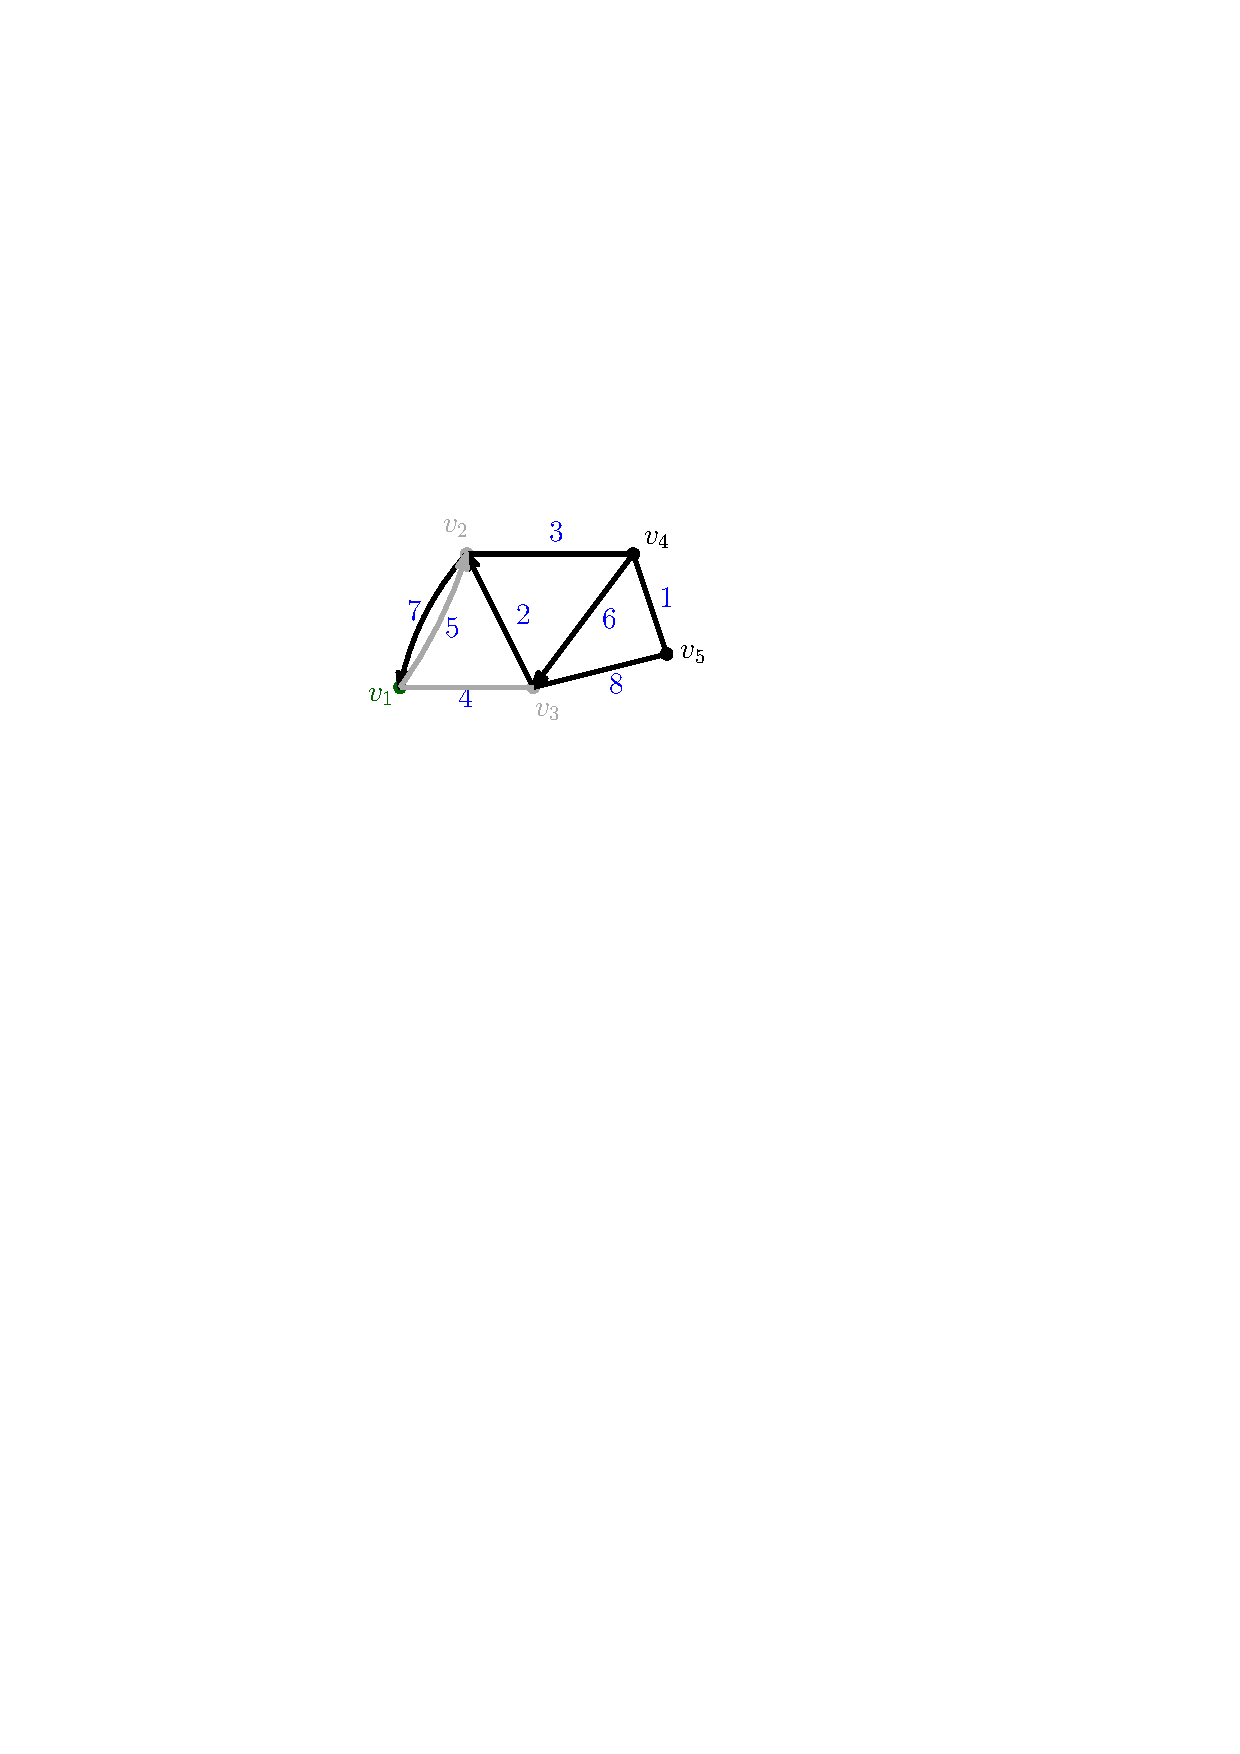
\includegraphics[width = \textwidth]{../media/dijkstra1.pdf} \\
\caption{1. Iteration}
\vspace{0.5cm}
\label{fig:dijkstra1}
\end{subfigure}
\begin{subfigure}{0.32\textwidth}
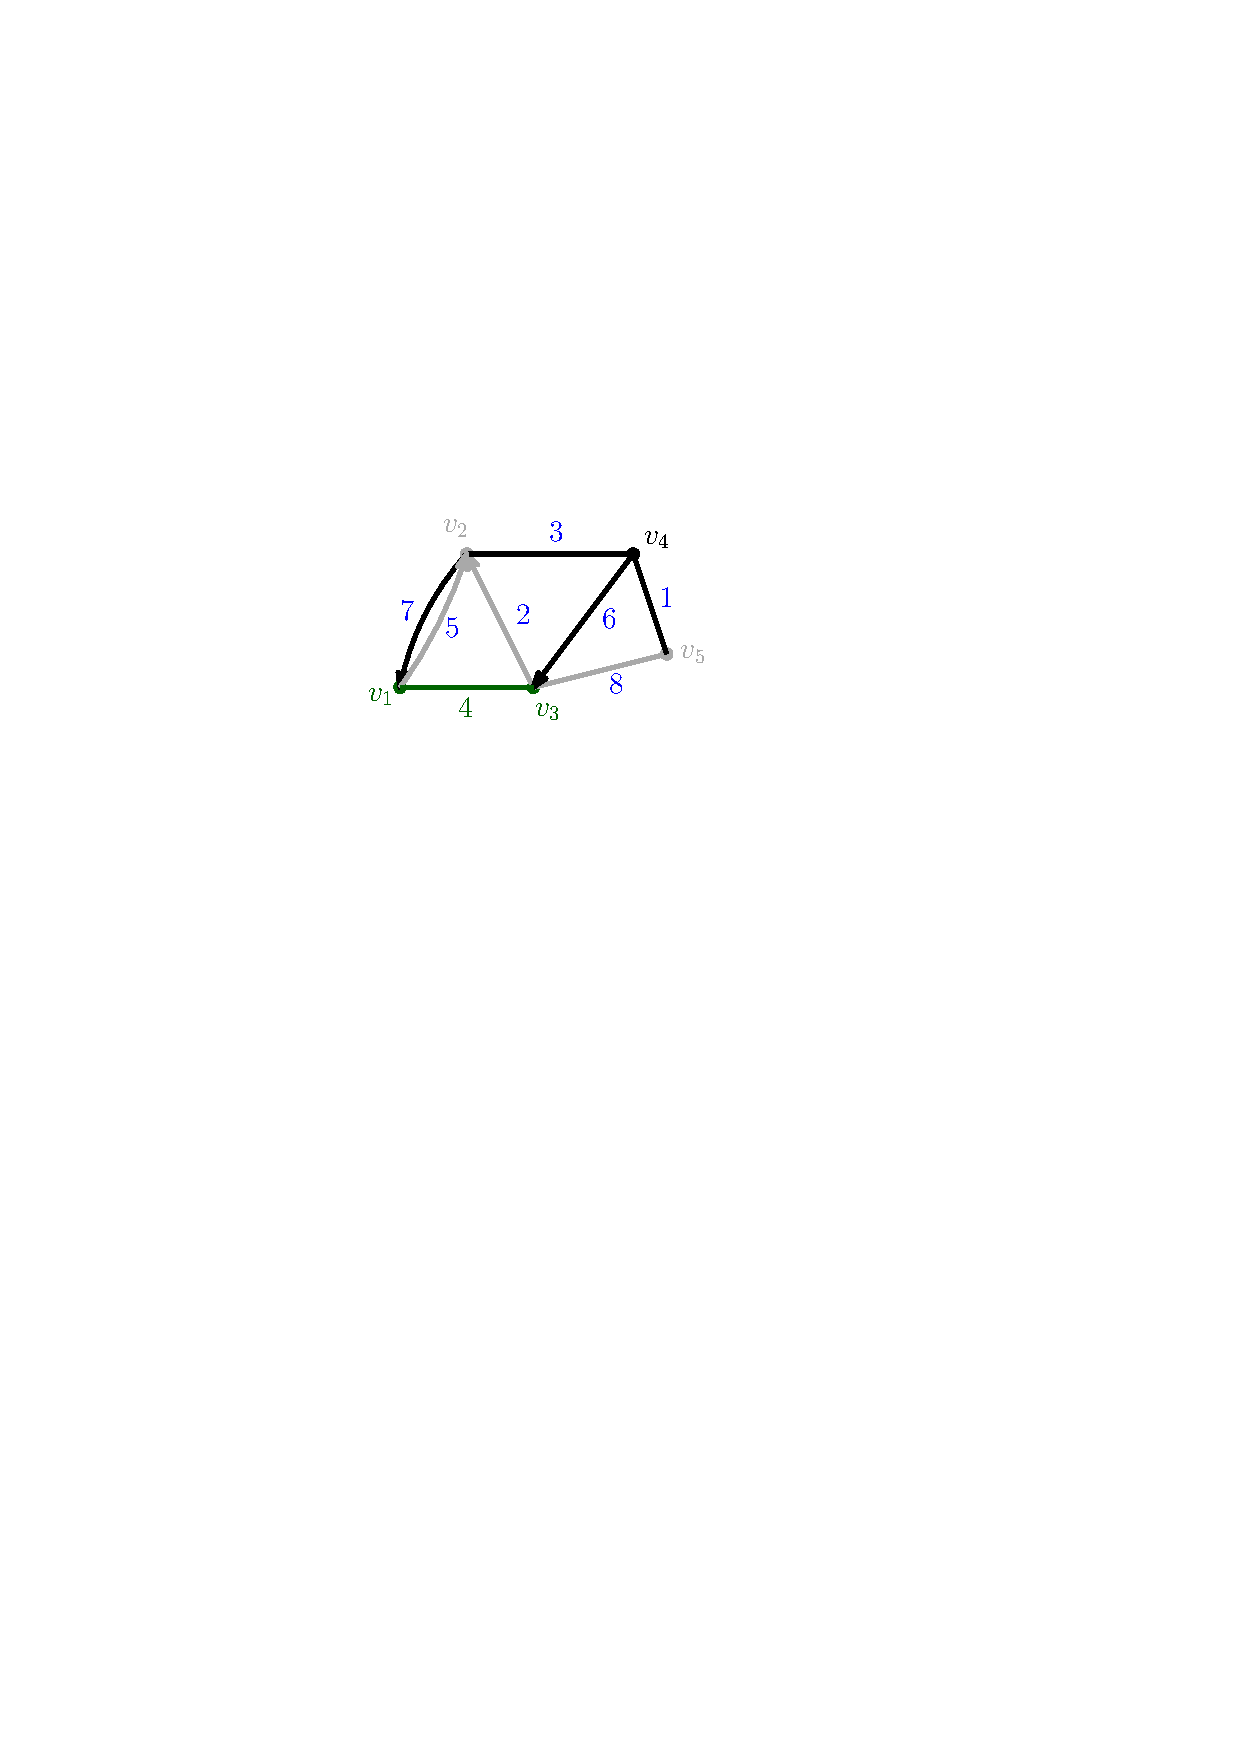
\includegraphics[width = \textwidth]{../media/dijkstra2.pdf} \\
\caption{2. Iteration}
\vspace{0.5cm}
\label{fig:dijkstra2}
\end{subfigure}
\begin{subfigure}{0.32\textwidth}
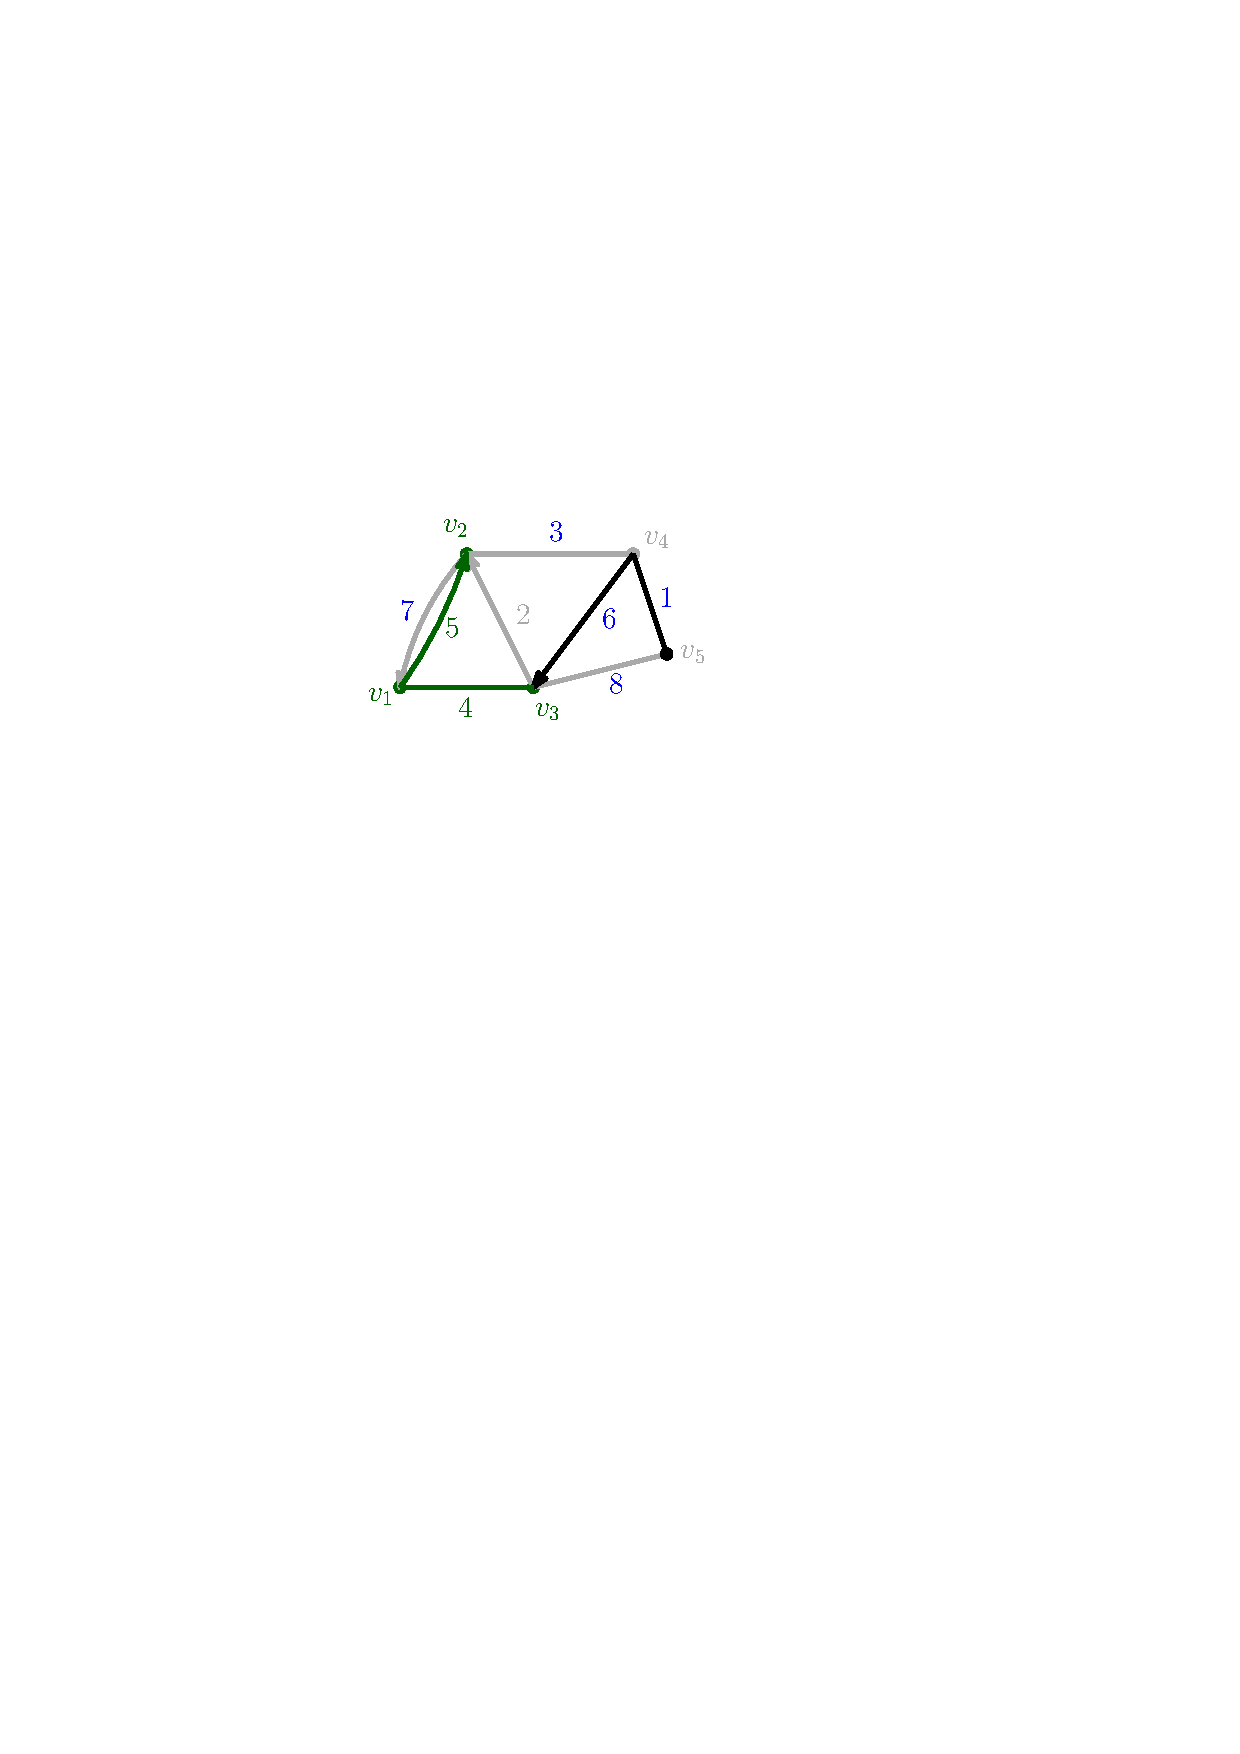
\includegraphics[width = \textwidth]{../media/dijkstra3.pdf} \\
\caption{3. Iteration}
\vspace{0.5cm}
\label{fig:dijkstra3}
\end{subfigure}
\begin{subfigure}{0.32\textwidth}
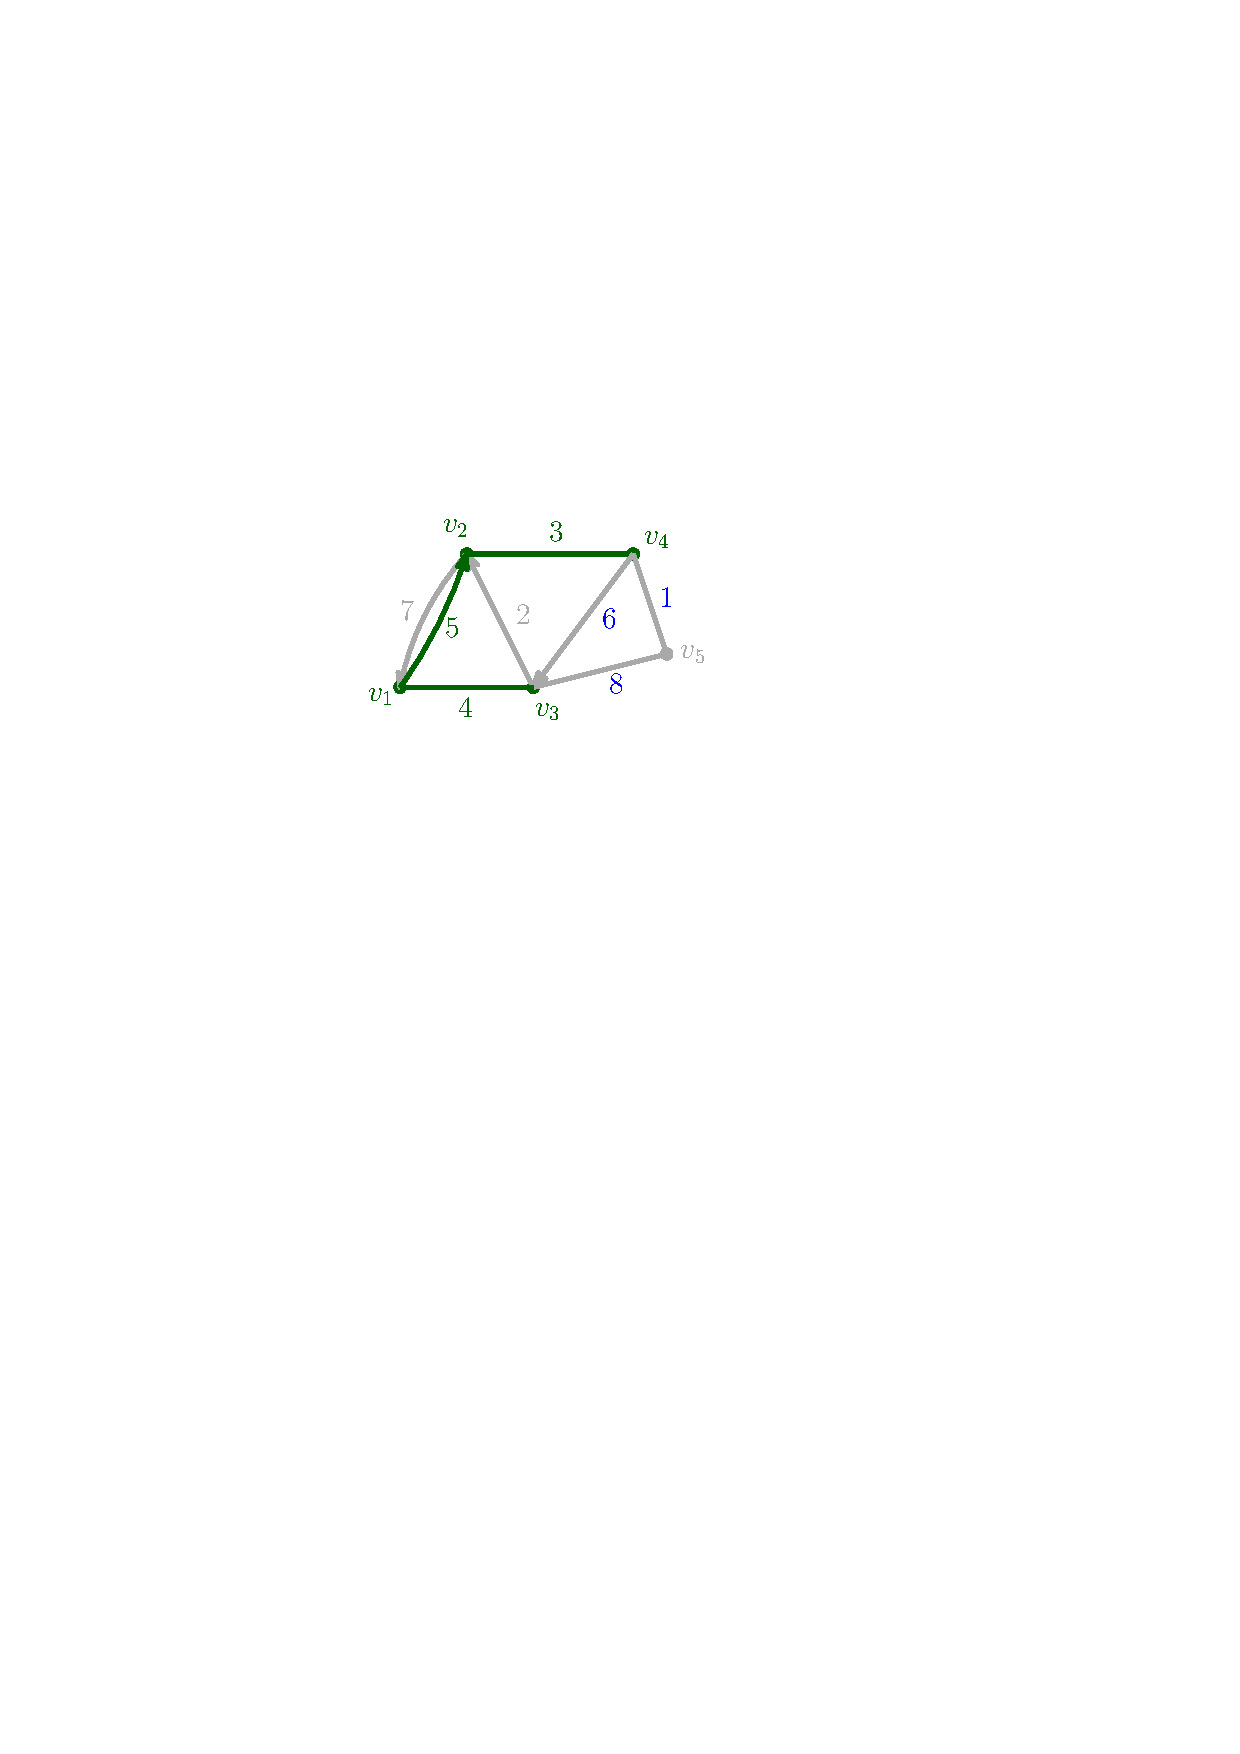
\includegraphics[width = \textwidth]{../media/dijkstra4.pdf} \\
\caption{4. Iteration}
\vspace{0.5cm}
\label{fig:dijkstra4}
\end{subfigure}
\begin{subfigure}{0.32\textwidth}
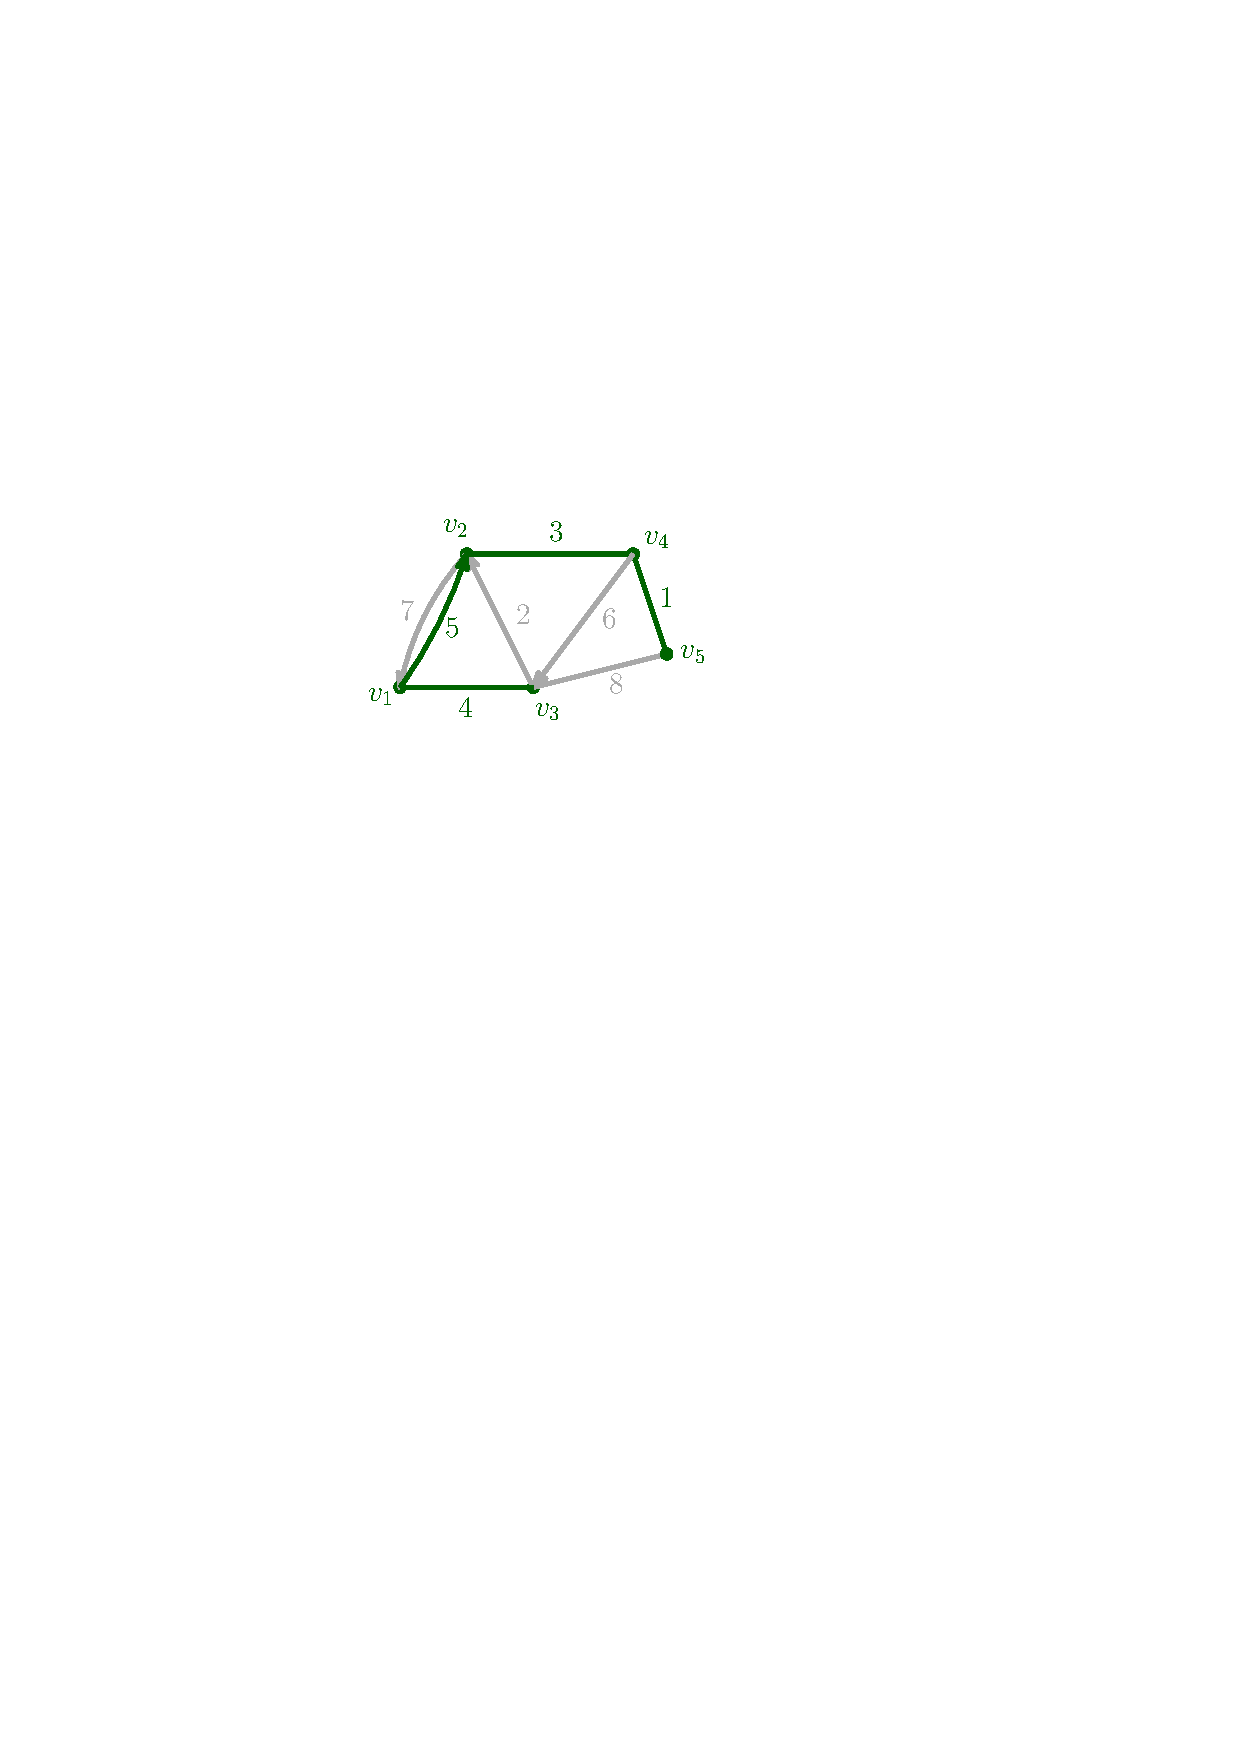
\includegraphics[width = \textwidth]{../media/dijkstra5.pdf} \\
\caption{5. Iteration}
\vspace{0.5cm}
\label{fig:dijkstra5}
\end{subfigure}
\caption{Kompletter Durchlauf eines Dijkstra Algorithmus}
\label{dijkstraIterations}
\end{figure}

\begin{table}{1\textwidth}
\label{tab:dijkstraLists}
\caption{$W_{s}$ und $K_{s}$ für jede Iteration aus Abb.~\ref{dijkstraIterations}
\begin{tabular}{r|l|l}

\multicolumn{1}{l}{} & \multicolumn{1}{|c}{$W_{s}$}                                                                        & \multicolumn{1}{|c}{$K_{s}$}                                                                                                                                \\ \hline
1.                               & \begin{tabular}[c]{@{}l@{}}$v_{2}:5(v_{1})$ $v_{3}:4(v_{1})$\end{tabular}  & $v_{1}: 0(v_{1})$                                                                                                                    \\ \hline
2.                               & \begin{tabular}[c]{@{}l@{}}$v_{2}:5(v_{1})$ $v_{5}:12(v_{3})$\end{tabular} & \begin{tabular}[c]{@{}l@{}}$v_{1}:0(v_{1})$ $v_{3}:4(v_{1})$\end{tabular}                                                          \\ \hline
3.                               & \begin{tabular}[c]{@{}l@{}}$v_{5}:12(v_{3})$ $v_{4}:8(v_{2})$\end{tabular} & \begin{tabular}[c]{@{}l@{}}$v_{1}:0(v_{1})$ $v_{3}:4(v_{1})$ $v_{2}:5(v_{1})$\end{tabular}                                       \\ \hline
4.                               & $v_{5}:9(v_{4})$                                                             & \begin{tabular}[c]{@{}l@{}}$v_{1}:0(v_{1})$ $v_{3}:4(v_{1})$ $v_{2}:5(v_{1})$ $v_{4}:8(v_{2})$\end{tabular}                    \\ \hline
5.                               & \multicolumn{1}{c|}{-}                                                       & \begin{tabular}[c]{@{}l@{}}$v_{1}:0(v_{1})$ $v_{3}:4(v_{1})$ $v_{2}:5(v_{1})$ $v_{4}:8(v_{2})$ $v_{5}:9(v_{4})$\end{tabular} \\
\end{tabular}
\end{table}



Damit wurde das \gls{ssp} gelöst und einen kürzeste Wege zu jeder Ecke des Graphen vom Startpunkt. Daraus ergibt sich auch die Lösung aller SPP für $s~$ zu jeder anderen Ecke aus $V~$. Es ist jedoch nicht sinnvoll für die Lösung eines \gls{spp} jedes mal das \gls{ssp} für den kompletten Graphen zu berechnen. Das liefert nicht nur viele irrelevante Ergebnisse sondern kostet auch mehr Berechnungsressourcen und Zeit. Daher gibt es unterschiedliche Möglichkeiten den Dijkstra Algorithmus zu beschleunigen.

\subsubsection{Speedup Techniken}

\paragraph*{Early Stopping:}
Der Algorithmus wird bisher jedes mal für den ganzen Graphen ausgeführt, obwohl oft nur die Route für einen kleinen Bruchteil des Graphen benötigt wird. Die einfachste Methode ist den Dijkstra zu stoppen, nachdem $z~$ erreicht wurde (~\ref{fig:normalD}). 


\paragraph*{Bidirectional Dijkstra:}
Beim bidirectional Dijkstra werden zeitgleich zwei Algorithmen nebeneinander ausgeführt. Einer auf $s~$ und einer auf $z~$ (auf einem umgekehrt gerichteten Graphen). Für beide Instanzen gibt es eine separate Warteschlange $W_{s}$ und $W_{z}$. Zu Beginn wird für jeden Startpunkt die initiale der umliegenden Ecken durchgeführt. Anschließend wird die Ecke mit der geringsten Distanz in beiden Warteschlangen markiert und aus der jeweiligen Warteschlange entfernt. Wird eine Ecke aus beiden Warteschlangen entfernt, werden $W_{s}$ und $W_{z}$ auf weitere übereinstimmende Ecken geprüft. Für jede Übereinstimmung wird die Distanz in beiden Instanzen Berechnet. Die Ecke ist Teil des kürzesten Weges wenn die Summe beider Distanzen minimal ist.\par
In der schematischen Abbildung ~\ref{fig:biD} wird die Einsparung gegenüber dem Early Stopping deutlich. Der graue Bereich muss nicht berechnet werden. Die Bearbeitungszeit lässt sich also theoretisch um die Hälfte reduzieren\footnote{In der Realität wir dieser Wert selten erreicht. Bei Graphen mit einer höheren Eckendichte in Nähe von $z~$ könnte die Bearbeitungszeit sogar größer werden. Allgemein wird aber ein signifikanter Vorteil erzielt.}.

\begin{figure}[h]
\centering
\begin{subfigure}{0.30\textwidth}
\centering
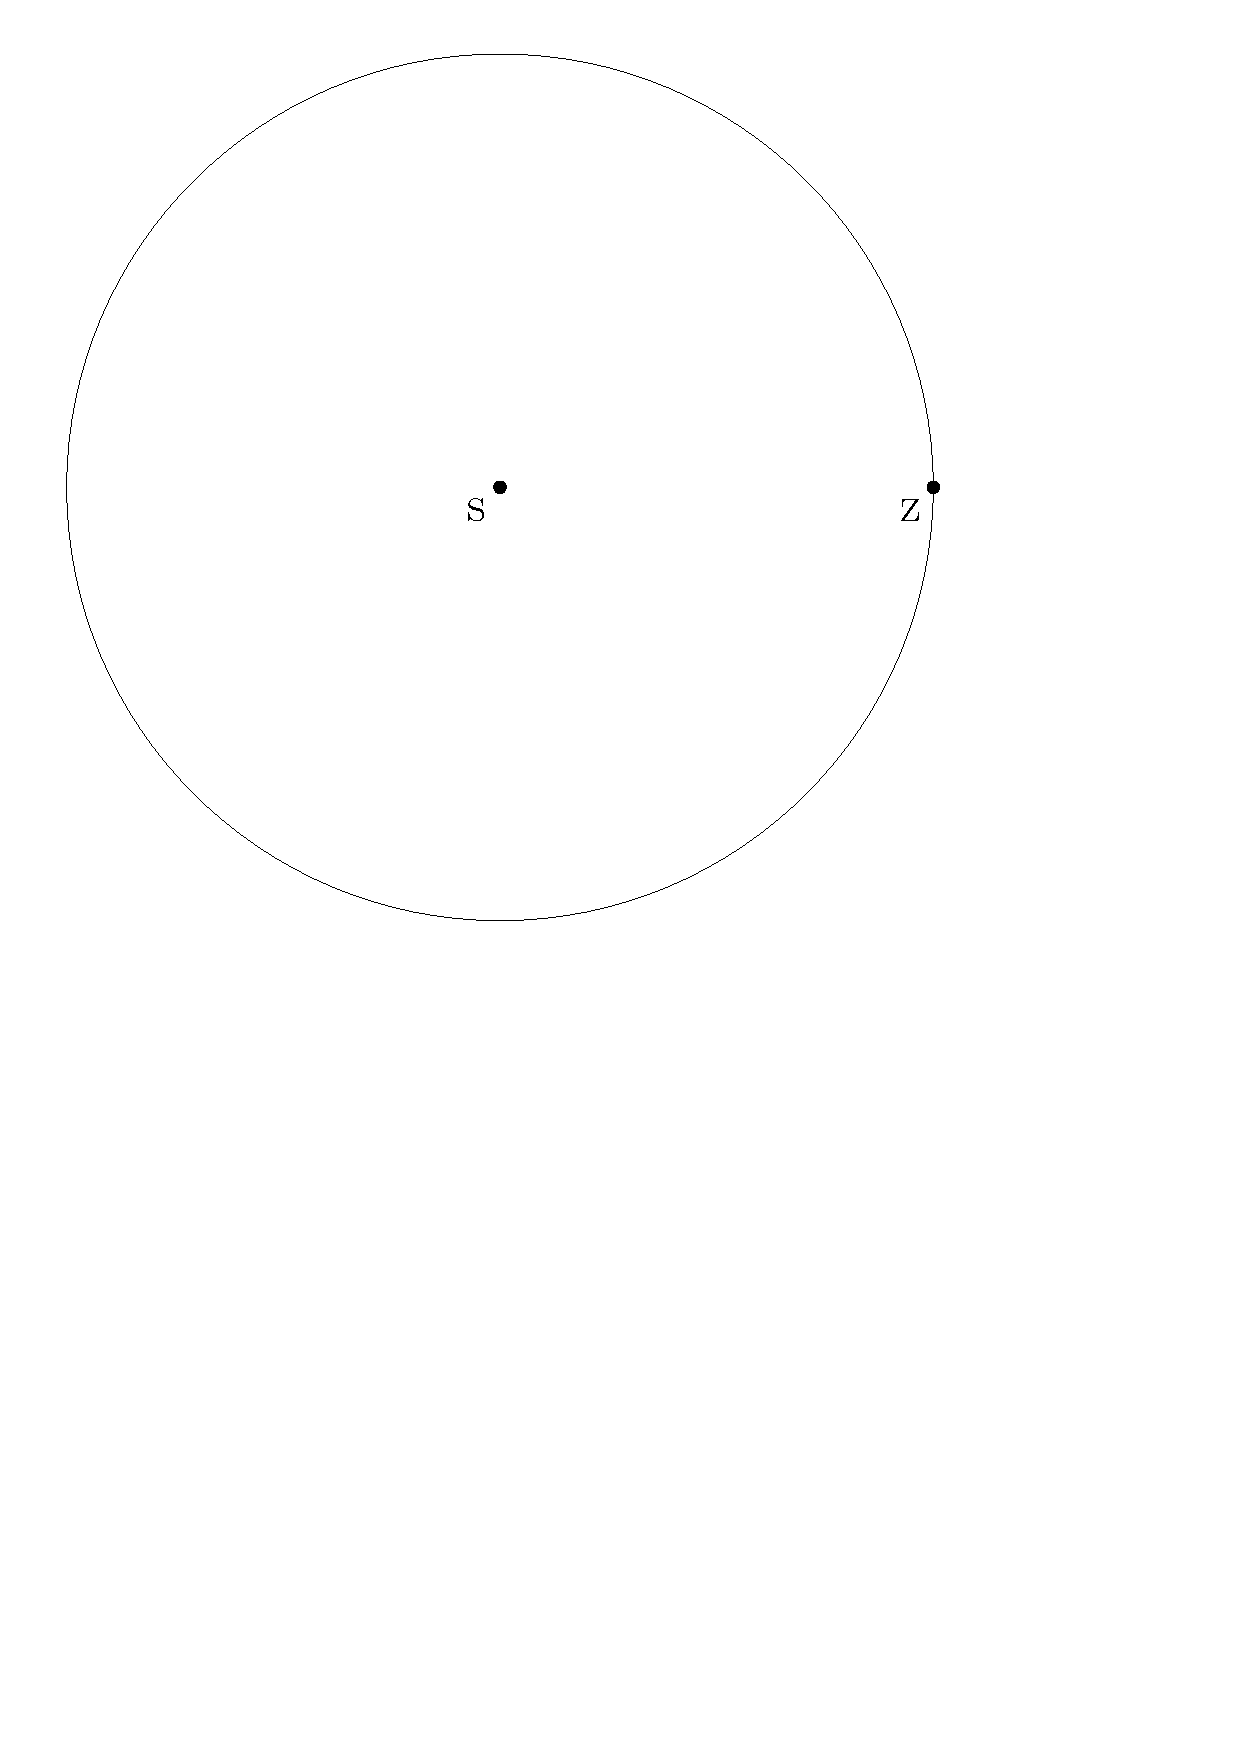
\includegraphics[width = \textwidth]{../media/normaldijkstra.pdf} \\
\caption{Early Stopping}
\label{fig:normalD}
\end{subfigure}
\begin{subfigure}{0.30\textwidth}
\centering
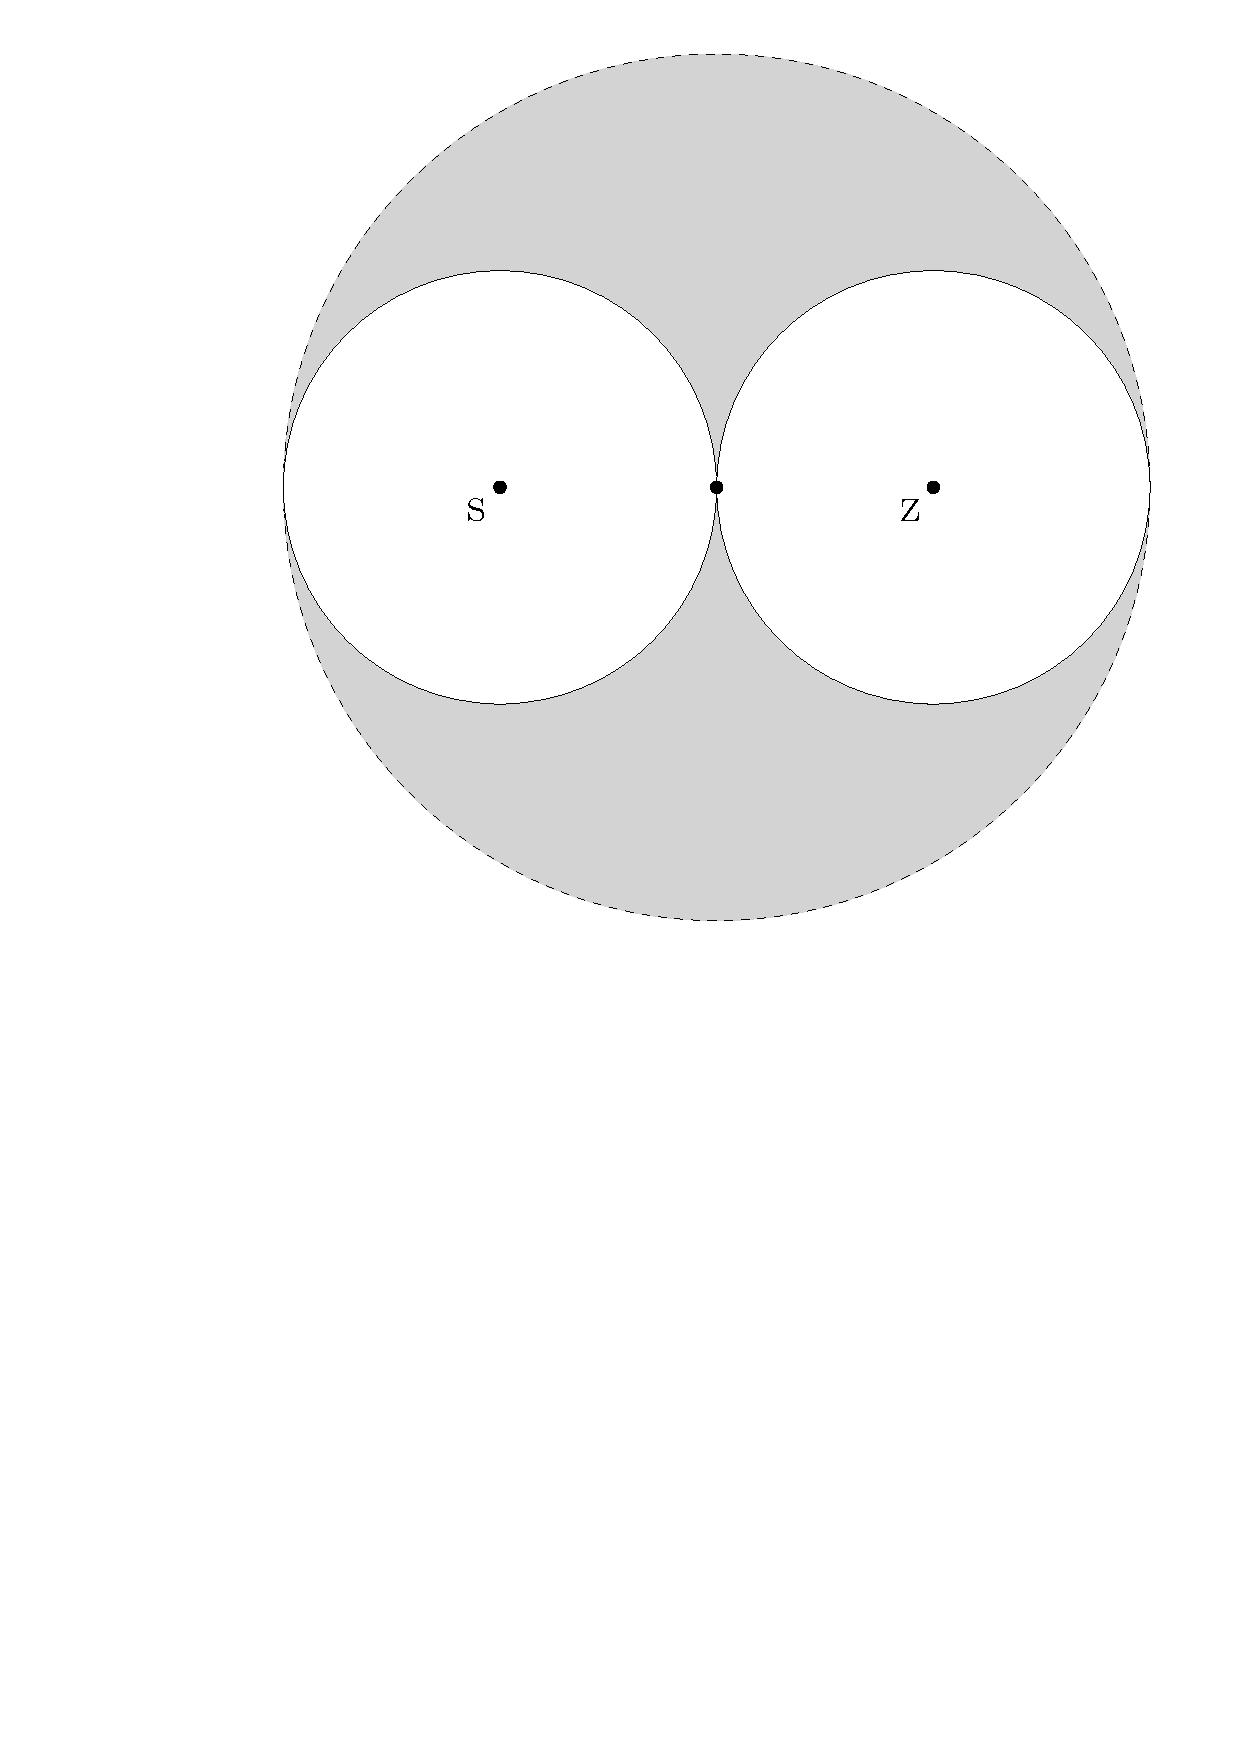
\includegraphics[width = \textwidth]{../media/bidijkstra.pdf} \\
\caption{Bidirectional D.}
\label{fig:biD}
\end{subfigure}
\begin{subfigure}{0.30\textwidth}
\centering
\vspace{1.1cm}
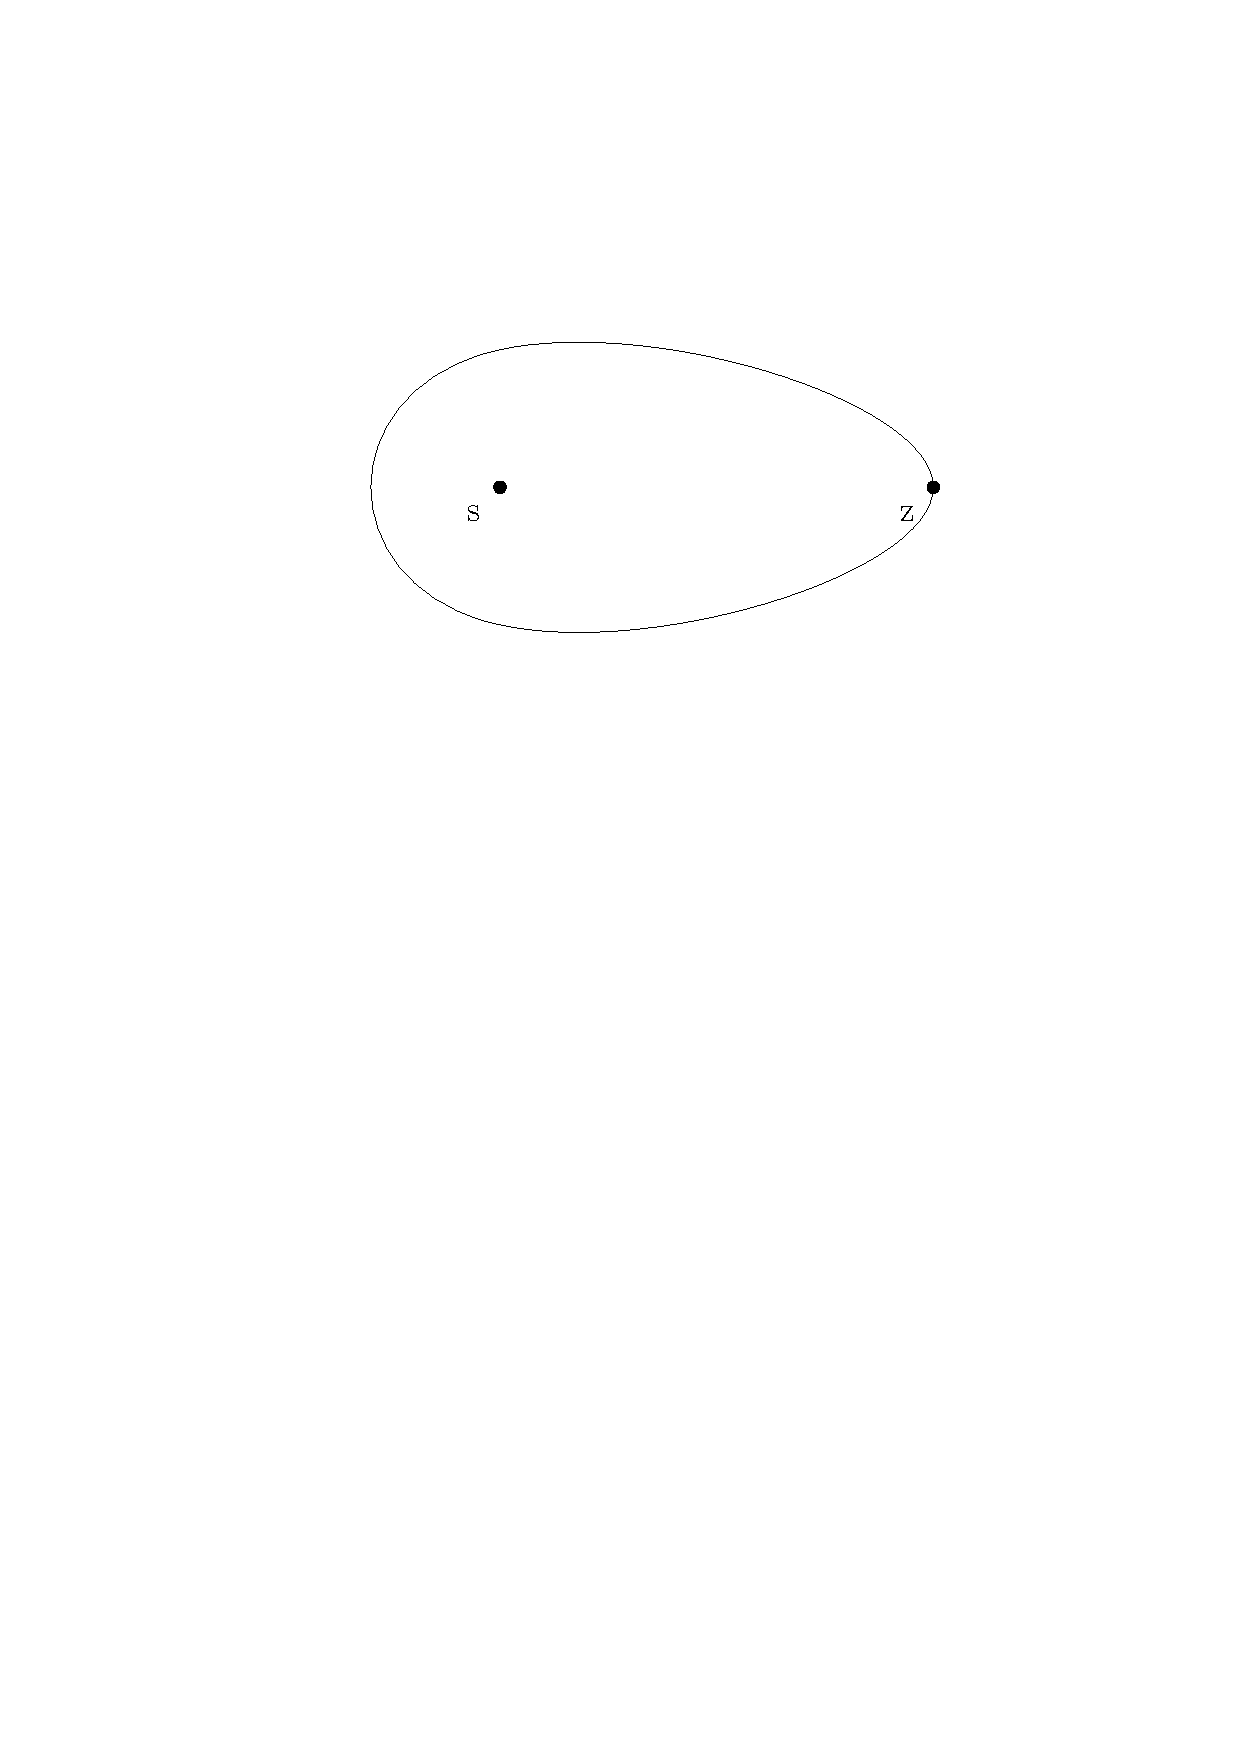
\includegraphics[width = \textwidth]{../media/stardijkstra.pdf} \\
\vspace{0.9cm}
\caption{A*}
\label{fig:starD}
\end{subfigure}
\caption{Speedup Techniken für den Dijkstra Algorithmus}
\label{speedup}
\end{figure}


\paragraph*{A*:}
Der $A*~$ Algorithmus ist eine Variante des Dijkstras die den Suchraum in Richtung der Zielecke lenkt. Es wird durch eine Funktion für jede Ecke die Distanz zum Ziel geschätzt. Diese wird mit den Kantengewichten verrechnet damit Ecken in Zielrichtung früher markiert werden. Die standardmäßig kreisförmige Ausbreitung des Dijkstras wird mit dem A* zu einem Oval gestreckt. Da der Zielpunkt so früher erreicht wird, müssen weniger Iterationen durchgeführt werden.

Diese und weitere Möglichkeiten sind in \cite[209--213]{kurt} ausführlich beschrieben.

\subsection{Isochronen Berechnung}

Isochronen sind Linien gleicher Zeit (griech.: \textit{iso} = gleich + \textit{chronos} = Zeit).

Wenn in einem gewichteten Graphen die Kanten die benötigte Zeit enthalten, um von einem Knoten zum nächsten zu gelangen, können damit Analysen zur Erreichbarkeit durchgeführt werden. Dazu wird ein \gls{ssp} für eine zentrale Ecke ~$z$ mit einem gegebenen Zeitlimit ~$t$ gelöst. 
Isochronen können mit unterschiedlichen Methoden berechnet werden. Das resultierende Objekt ist immer ein Polygon, welches jeden in gegebenem Zeitlimit erreichbaren Punkt beinhaltet.


\subsubsection{Gitterbasierter Ansatz}

Beim \textit{Marching Squares} Algorithmus wird um das Zentrum ein Gitter über dem Graphen gebildet (~\ref{fig:grid1}). Die Eckpunkte des Gitters erhalten dabei die Werte des nächsten Punktes auf dem Graphen(~\ref{fig:grid2}). Anschließend werden auf den Kanten des Gitters diejenigen Punkte markiert, bei denen der Wert mit dem gesuchten Zeitlimit übereinstimmt. In Abbildung ~\ref{fig:grid3} wurde das für die Werte $t=5$ und $t=10$ durchgeführt. Die markierten Punkte werden verbunden und bilden schließlich die Isochrone.

\begin{figure}[h]
\centering
\begin{subfigure}{0.47\textwidth}
\centering
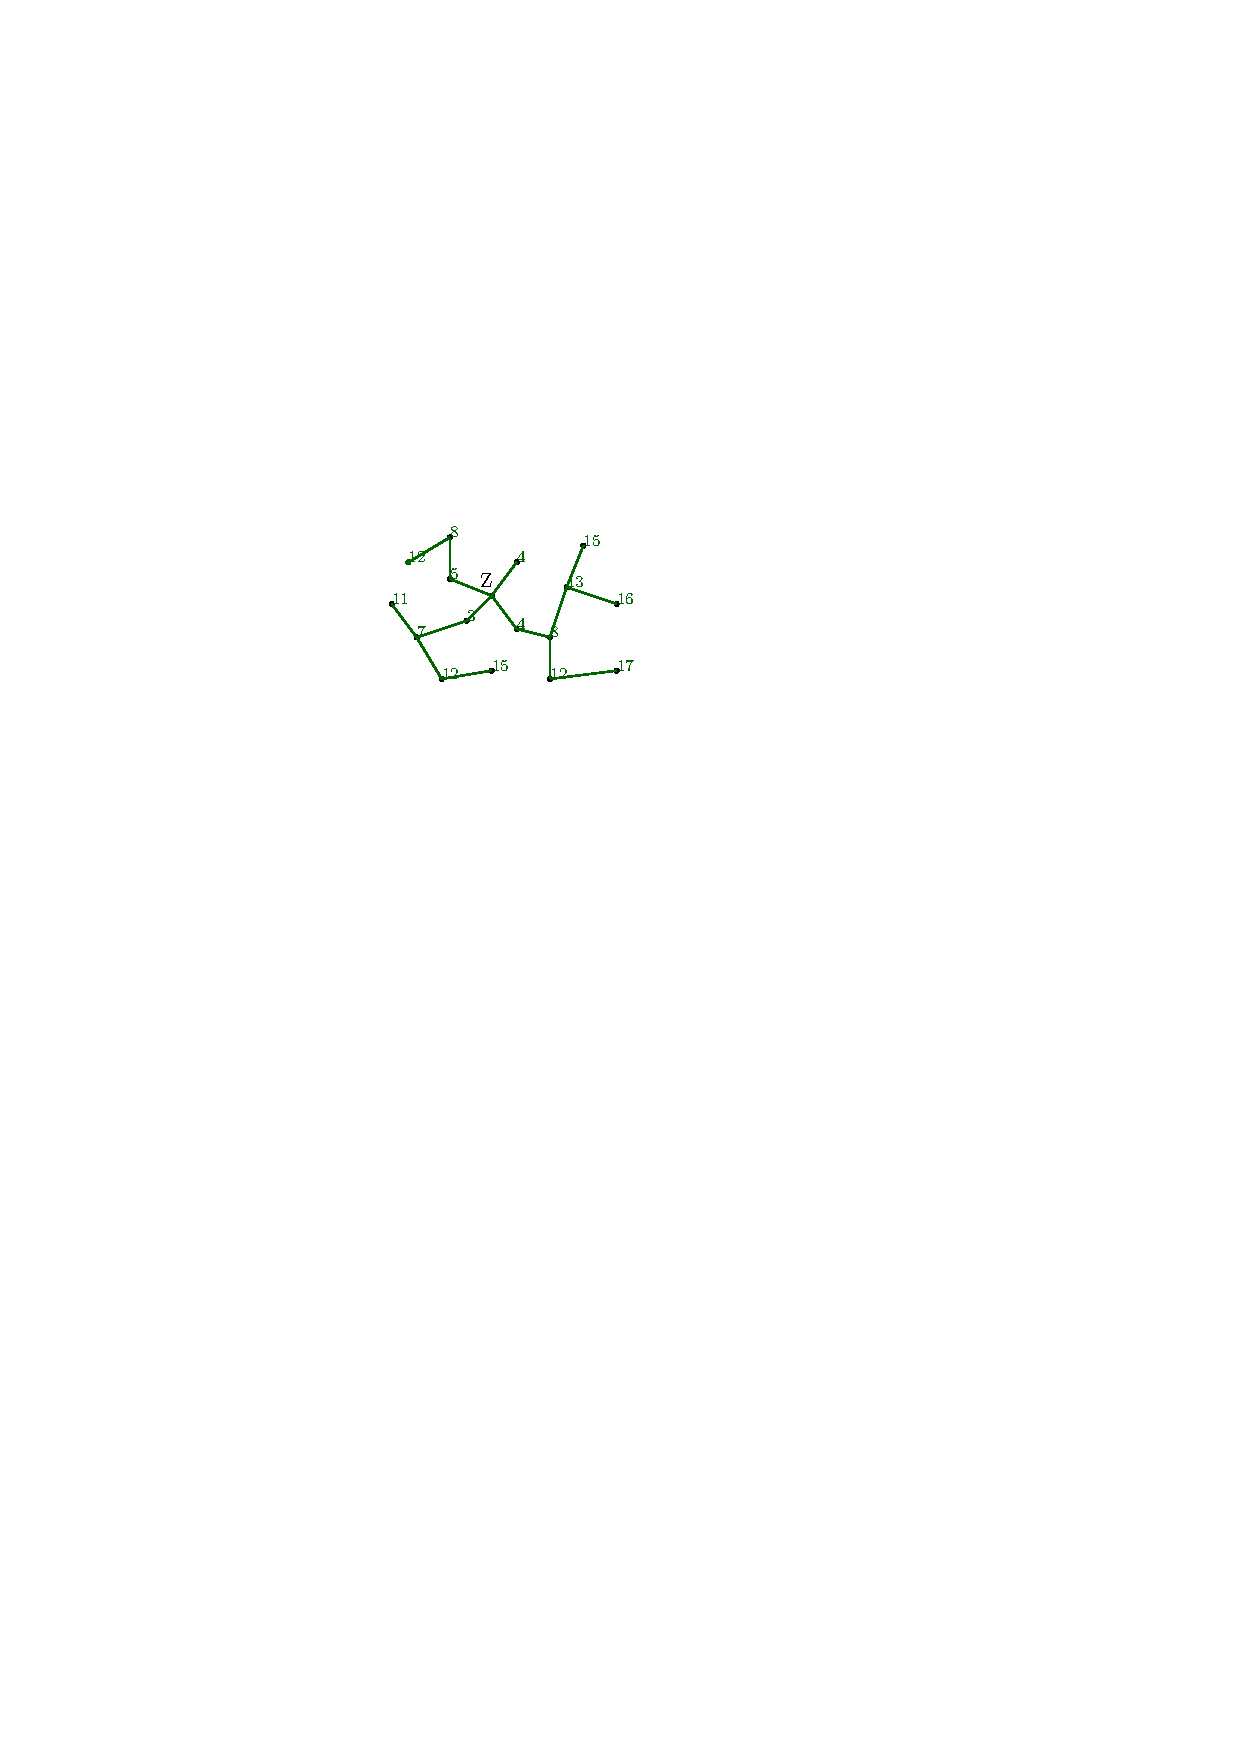
\includegraphics[width = \textwidth]{../media/grid.pdf} \\
\caption{Basis Graph mit kürzesten Wegen}
\vspace{0.3cm}
\label{fig:grid1}
\end{subfigure}
\begin{subfigure}{0.47\textwidth}
\centering
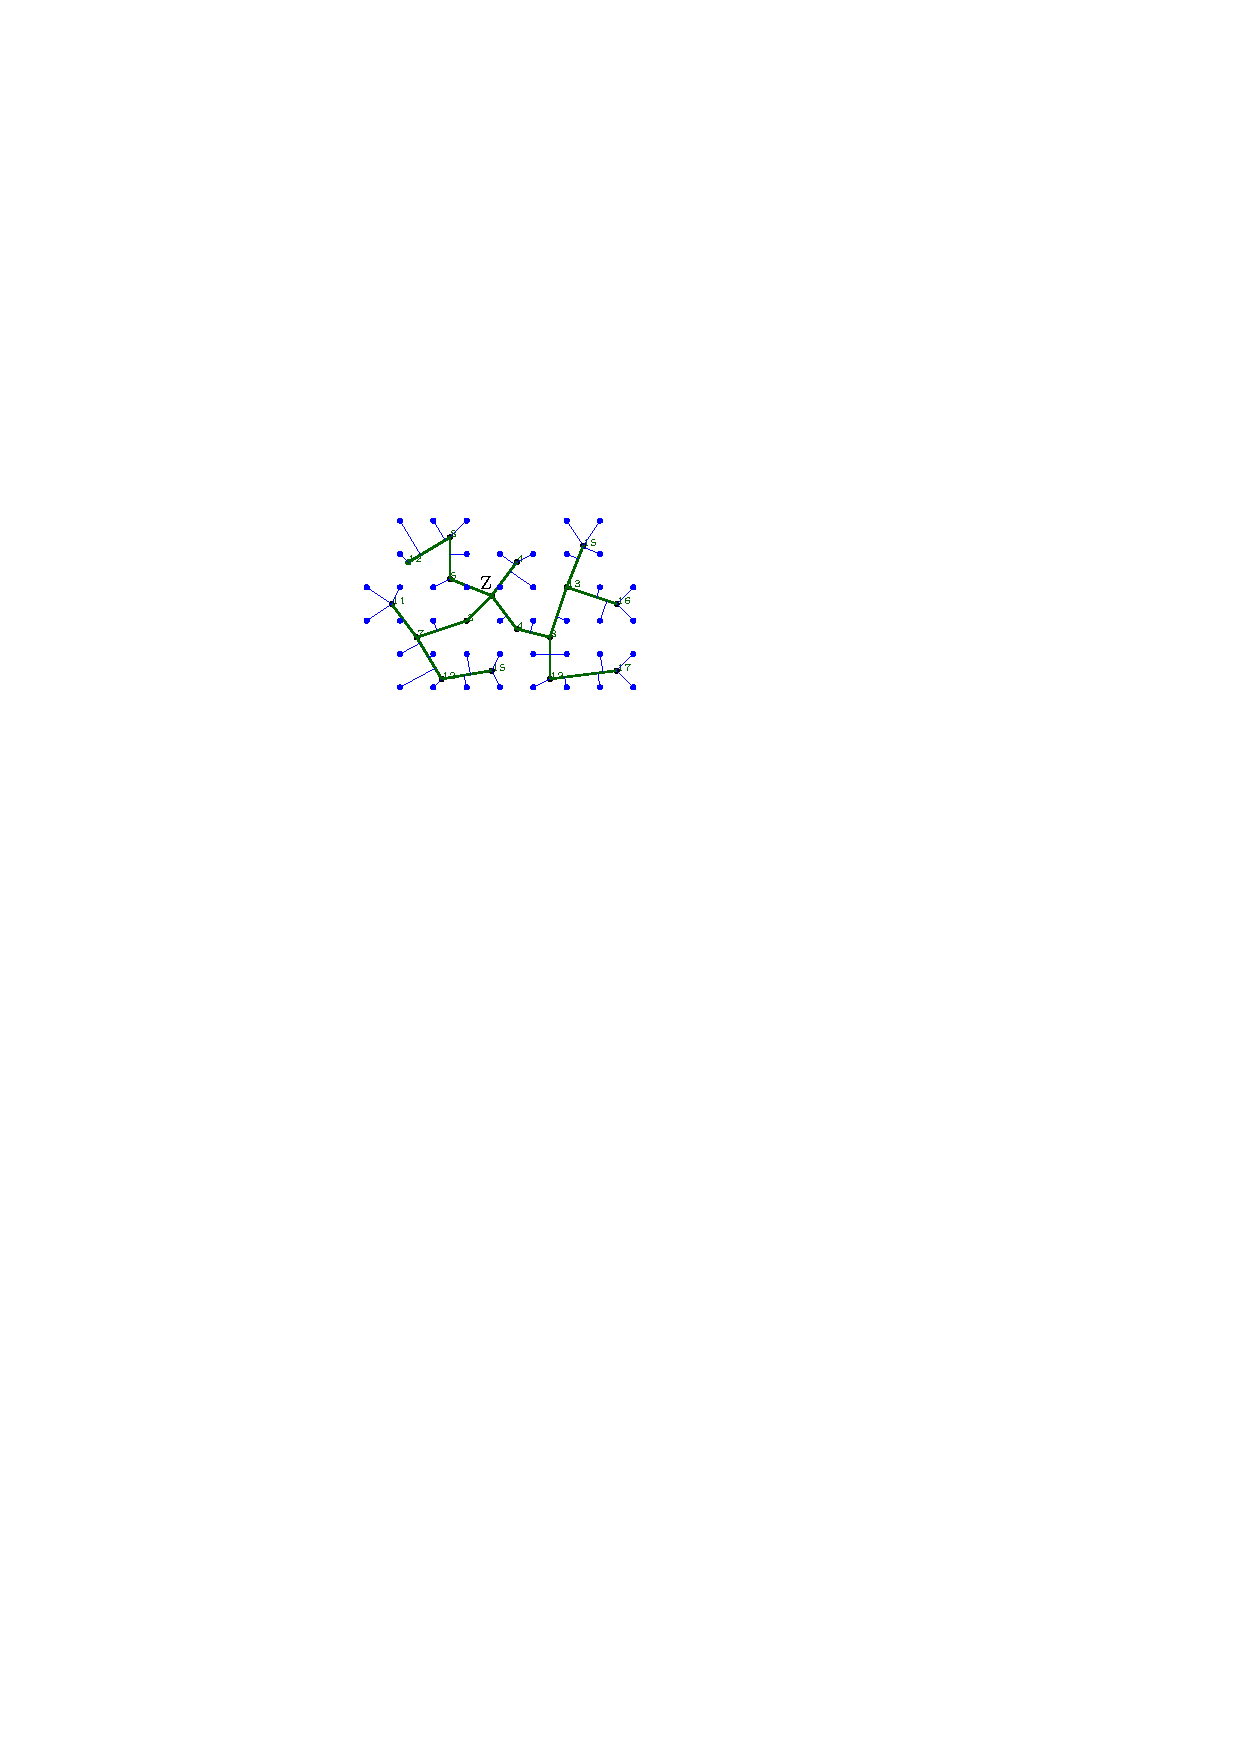
\includegraphics[width = \textwidth]{../media/gridsnap.pdf} \\
\caption{Gitterbildung}
\vspace{0.3cm}
\label{fig:grid2}
\end{subfigure}
\begin{subfigure}{0.44\textwidth}
\centering
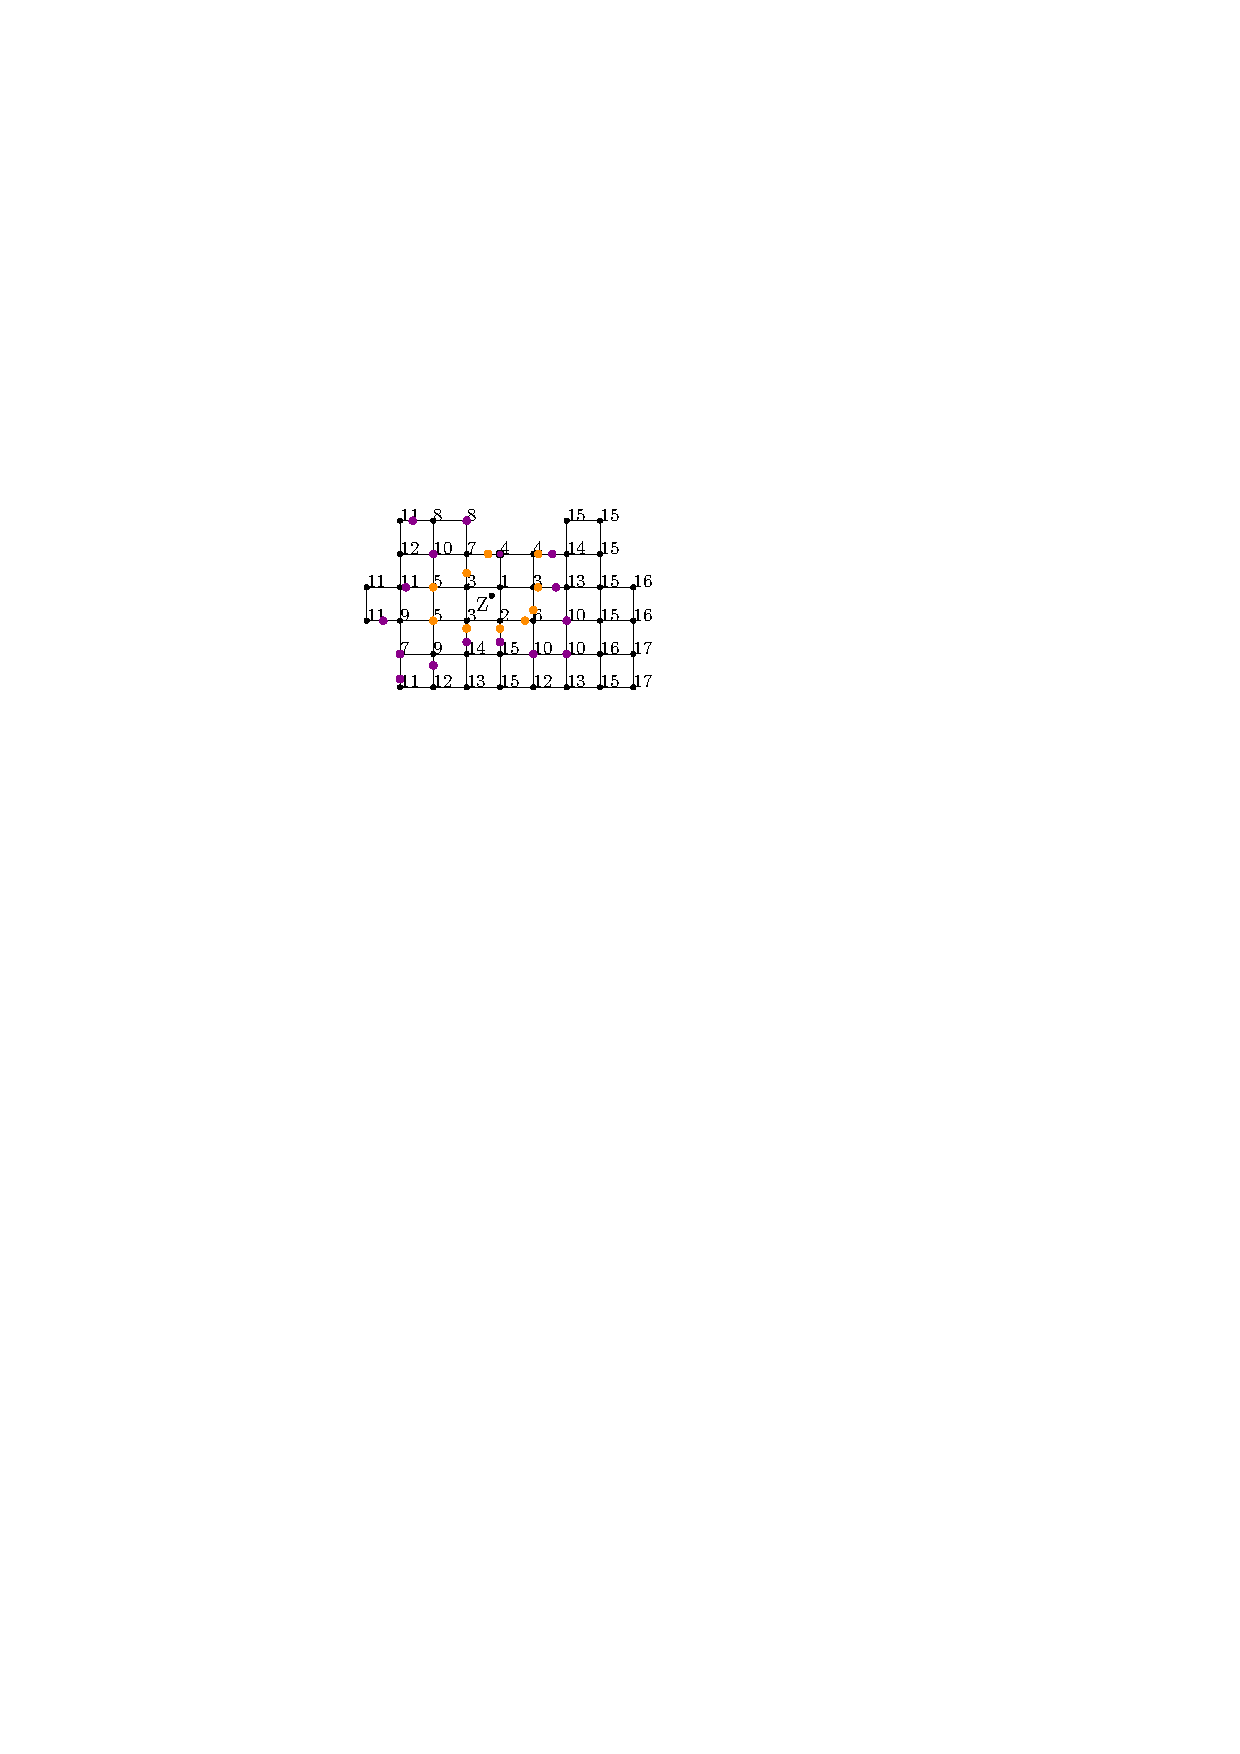
\includegraphics[width = \textwidth]{../media/gridedge.pdf} \\
\caption{Kantenmarkierung}
\label{fig:grid3}
\end{subfigure}
\begin{subfigure}{0.47\textwidth}
\centering
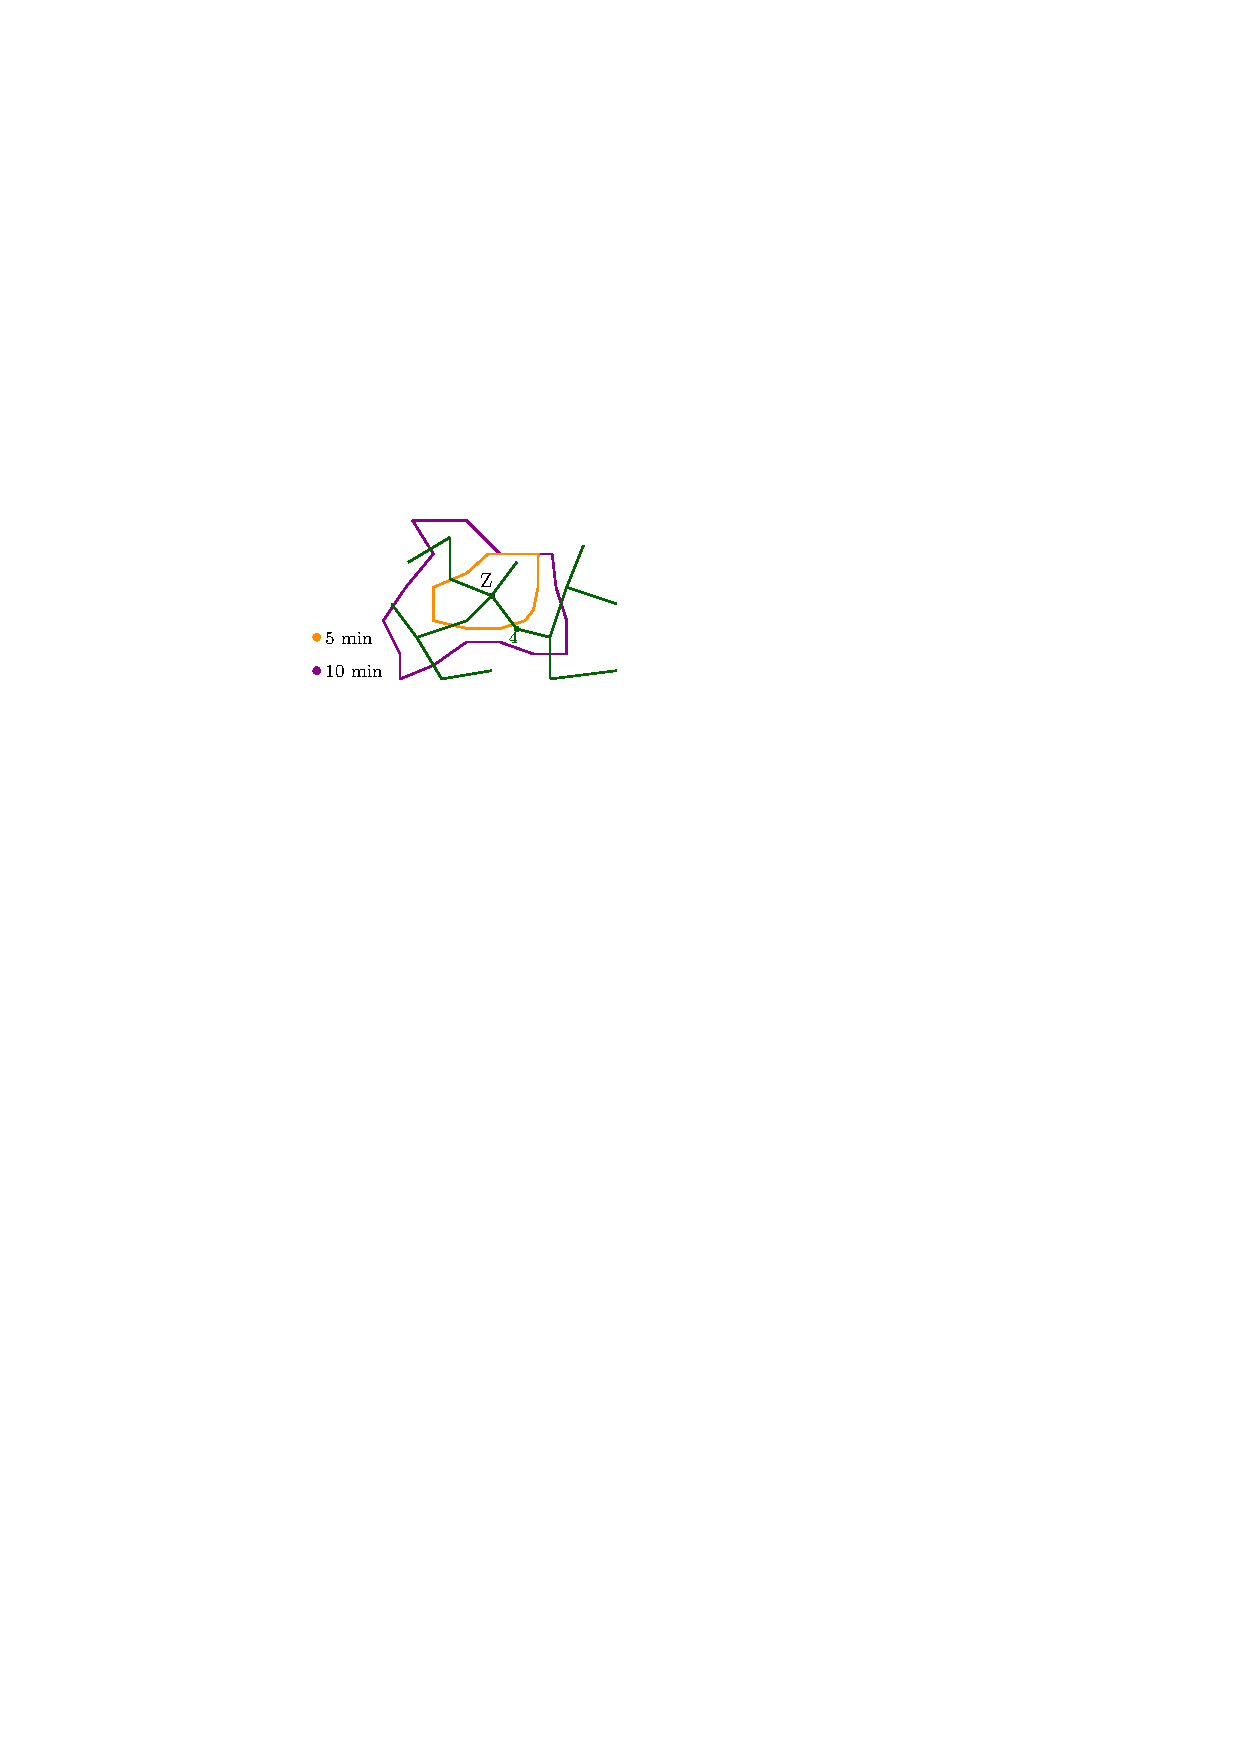
\includegraphics[width = \textwidth]{../media/gridiso.pdf} \\
\caption{Resultierende Isochrone}
\label{fig:grid4}
\end{subfigure}
\caption{Marching Squares Algorithmus}
\label{grid}
\end{figure}

Der Vorteil dieses Algorithmus ist, dass die Maschengröße des Gitters angepasst werden kann. 
Bei sehr kleinen Maschen liefert der Algorithmus ein sehr genaues Ergebnis. 
Allerdings werden dabei mehr Ressourcen zur Berechnung gebraucht. 
Daher können nur kleine Gebiete und geringe Zeitlimits berechnet werden. 
Bei weiten Maschen ist der Algorithmus dagegen sehr schnell und kann große Distanzen und lange Zeitspannen berechnen. 
Das Ergebnis ist dementsprechend aber auch ungenauer. 
Auch in Abbildung ~\ref{fig:grid4} wurde die Größe der Maschen unglücklich gewählt. 
Eine Ecke mit Abstand 4 Minuten vom Zentrum liegt dadurch außerhalb der 5-Minuten-Isochrone.

\subsubsection{Dreiecksvermaschung}
\cite{isochrones} beschreiben ein anschauliche Methode um Isochronen zu berechnen. 
Nach der Lösung des \gls{ssp}s werden den Ecken des Graphen die geographische Koordinate der repräsentierten Kreuzung zugeteilt. Die Kanten werden nicht benötigt und daher entfernt. 
Es liegt also eine 3D-Punktwolke vor. 
Jeder Ecke wird nun die benötigte Zeit zugewiesen, mit der diese zu erreichen ist. 
Anschließend werden die Ecken nach dem Delaunay Triangulationsverfahren vermascht. 
Es entsteht eine Art Trichter mit der Startecke als Tiefpunkt auf der Höhe Null. 
Wird dieser Trichter auf Höhe des Zeitlimits geschnitten, entsprechen von oben betrachtet die Randkanten des Trichters der Isochrone.


\subsubsection{Formenbasierter Ansatz}
Die Implementierung des \gls{ors} zur Berechnung von Isochronen verwendet ist einen Form-basierten Ansatz. Zuerst werden mit dem in Kapitel ~\ref{sec:dijkstra} bereits ausführlich erklärten Dijkstra Algorithmus alle in gegebener Zeit erreichbaren Kanten markiert. Anschließend werden die geographischen Punkte (Pillar Nodes) aus der WayGeometry der Kante extrahiert (Siehe Kapitel ~\ref{sec:osmgraph} auf Seite ~\pageref{sec:osmgraph}). Um jeden der extrahierten Punkte wird ein kreisförmiger Pufferbereich gelegt. Dadurch können nahe beieinanderliegende Punkte übersprungen werden. Mit den verbleibenden Punkten wird eine Punktwolke generiert. Auf diese Punktwolke wird nun der Alpha-Shape Algorithmus(Zitat) angewandt um die Isochrone als Hülle um die erreichbaren Wegsegmente zu zeichnen.
(Abb. Pictures shape based stuff)
Dieser Ansatz liefert präzise Ergebnisse bei schnellen Berechnungszeiten. Die Verwendung der Alpha-Shapes verhindert allerdings die Möglichkeit der Darstellung von nicht erreichbaren 'Löchern' innerhalb der Isochronen.

\newpage
\section{Generierung des Routing-Profils/Methodik?}
Die Grundsätzlichen Überlegungen beruhen, wie in der Einleitung bereits erwähnt, auf den Notstandsvollmachten durch §35 Absatz 1 der StVO für Einsatzfahrzeuge des Rettungsdienstes, der Feuerwehr und der Polizei. Demnach dürfen sich Einsatzfahrzeuge im Notfall über die Vorschriften der StVO hinwegsetzen. Die Frage ist allerdings in wieweit von diesen Rechten im Ernstfall Gebrauch gemacht werden kann. Um dieser Sache auf den Grund zu gehen, wurde ein Fragenkatalog für die \gls{ffl} zusammengestellt. Dieser wurde als Datei auf Google Docs gespeichert und ist auch weiterhin verfügbar(Link im \ref{sec:anhang}). Die Fragen wurden mit Hinblick auf die OSM Datenstruktur und das vorhandene ORS Backend gewählt. Die Antworten der \gls{ffl} sind hier sinngemäß wiedergegeben. Die wörtlichen Antworten sind dem Google Dokument im Anhang zu entnehmen.

\subsection{Informations Erhebung}

\paragraph*{1. Maße der Fahrzeuge:}
\label{frage1}
Die Dimensionen des Fahrzeuges sind limitierende Faktoren für bestimmte Wegsegmente. Manche Brücken halten nur ein bestimmtes Gewicht aus und ein Tunnel hat nur eine gewisse Höhe.
Hier stützt sich das ORS Backend auf Restriktionen durch die \gls{osm}-Tags: \lstinline!maxlength, maxwidth, maxheight, maxweigth! und \lstinline!maxaxleload! Von der \gls{ffl} wurde als wichtigstes Fahrzeug Löschfahrzeuge der Klasse LF8, LF8/6 und MLF mit folgenden Daten angegeben:
- Länge: 7 Meter
- Breite: 2,5 Meter
- Höhe: 3 Meter
- Gewicht: 7,5 Tonnen
- Achslast: k.A.\todo{ask Stefan} Tonnen 

\paragraph*{2. Maximale Geschwindigkeiten auf unterschiedlichen Straßentypen:}
\label{frage2}
Es kann nicht auf jeder Straße mit maximaler Geschwindigkeit des Fahrzeugs gefahren werden. Deswegen werden für jede Kante des Graphen Geschwindigkeitsmaxima definiert.
Dabei wird auf einen Standardwert für den Straßentyp, die \textit{Values}(Werte) des \gls{osm} \textit{Keys} (Schlüssel) \lstinline!highway!, zurückgegriffen.
Tabelle ~\ref{tab:speedinfo} zeigt die bisherigen Standardgeschwindigkeiten für das Schwerfahrzeug-Profil des \gls{ors} zusammen mit den vorgeschlagenen Werten der \gls{ffl} in Klammer.
Es wurde darauf hingewiesen, dass die 80km/h auf Autobahnen nur gelten wenn kein Stau besteht. Im Fall eines Staus wäre laut \gls{ffl} auch die Anfahrt auf der Gegenfahrbahn bzw. entgegen der Verkehrsrichtung auf der gleichen Bahn interessant.
Auf Wirtschafts-, Wald- und Wiesenwegen mit dem Key-Value-Paar  \lstinline!highway=track! kann zusätzlich der Zustand des Weges mit dem Tag \lstinline!waytype! beschrieben werden. Die bisherigen und vorgeschlagenen Geschwindigkeit für die jeweiligen Values sind in Tabelle \ref{tab:speedinfotrack} zu sehen.

Genaue Informationen zu einzelnen Tags können der \gls{osm} Wikipedia (\ref{osmwiki}) entnommen werden.

\begin{figure}
\label{tab:speedinfo}
\caption{Standardgeschwindigkeiten für unterschiedlichen \lstinline!highway! Values}
\begin{tabular}{|l|c|}
\multicolumn{1}{1}{\lstinline!highway! Value}  & \multicolumn{1}{|c|}{HGV-Profil} 
\hline //
\multicolumn{2}{|l|}{\textit{Autobahnen}} //
\lstinline!motorway! (Autobahn) & 80 //
\lstinline!motorway\_link! (Autobahn-Zubringer) & 50 //
\lstinline!motorroad! () & 80 //
\lstinline!trunk! (Schnellstraße) & 80 //
\lstinline!trunk\_link! (Zubringer zu Schnellstraße) & 50 //
\multicolumn{2}{|l|}{\textit{Siedlungen}} //
\lstinline!primary! (Bundesstraßen) : 60(80) //
\lstinline!primary!\_link  : bisher 50 //
\lstinline!secondary! (Landes-/Staatsstraßen) : 80 bisher 60 //
\lstinline!secondary\_link!  : bisher 50 //
\lstinline!tertiary! (Kreisstraßen) : 80 bisher 60 //
\lstinline!tertiary!\_link  : bisher 50 //
\lstinline!unclassified! (Nebenstraße (oft keine Mittellinie))  : bisher 60 //
\lstinline!residential! (Straße an und in Wohngebieten) : bisher 50 //
\lstinline!living\_street! (''Spielstraße'')  : bisher 10 //
\lstinline!service! (Erschließungsstraße) : bisher 20 //
\lstinline!road! (unbekannte Straße) : bisher 20 //
\lstinline!track! (Wald-/Feldweg) : bisher 15 //
\end{tabular}
\end{figure}

\begin{figure}
\label{tab:speedinfotrack}
\caption{Standardgeschwindigkeiten für unterschiedlichen \lstinline!tracktype! Values}
\begin{tabular}{|l|c|}
\multicolumn{1}{1}{\lstinline!tracktype! Value}  & \multicolumn{1}{|c|}{HGV-Profil} 
\hline
\lstinline!grade1!(Wasserfester Belag) & 20(25)     //
\lstinline!grade2!(Wassergebundene Decke) & 15    //
\lstinline!grade3!(Befestigter oder ausgebesserter Weg) & 10(15)  //
\lstinline!grade4!(Unbefestigter Weg) & 5(10)     //
\lstinline!grade5!(Unbefestigter Weg) & 5     //
\end{tabular}
\end{figure}

// highways (Autobahnen)
 bisher 80 (Kommt natürlich auf den Verkehr und dann auf die Rettungsgasse an) (Wenn es nur als Zubringer verwendet wird geht es wenn kein Stau ist schon. Ist der Einsatzort auf der Autobahn (VU oder ähnliches) Kommt es natürlich zu einem Stau, dann langsamer. Hier wäre vielleicht ein Schalter interessant auch auf der Gegenfahrbahn anfahren zu können auf der gleichen Höhe, bzw. auch gegen die Verkehrsrichtung auf der gleichen Bahn.


\paragraph*{3. Dürfen vorgegebene Geschwindikeiten (Bsp. 30er Zone/ Tempolimit 70 etc) überschritten werden?}
\label{frage3}
Manchmal sind besondere Geschwindikeitsrestriktionen, wie zum Beispiel Tempo-30-Zonen vorhanden.  In Tempo-30-Zonen darf 50 km/h und in Spielstraßen darf 20 km/h gefahren werden. Dabei ist immer noch auf die Unversehrtheit der anderen Verkehrsteilnehmer (vor allem Kinder) zu achten.

\paragraph*{4. Dürfen Gewicht und/oder Achslast für Straßen mit Vorgabe überschritten werden?}
\label{frage4}

Es dürfen Straßen benutzt werden die zum Beispiel wegen einer folgenden Brücke auf 7,5 Tonnen beschränkt sind. Um die Brücke selbst zu nutzen ist allerdings lokales Wissen über die tatsächliche Tragfähigkeit notwendig. 
Allgemein müssen bei Zu- oder Durchfahrten für die Feuerwehr die Aufstellflächen und die Bewegungsflächen so befestigt sein, dass sie von Feuerwehrfahrzeugen mit einer Achslast bis zu 10 t und einem zulässigen Gesamtgewicht bis zu 16 t befahren werden können.

\paragraph*{5. Dürfen Einbahnstraßen in Entgegengesetzter Richtung durchfahren werden?}
\label{frage5}

Einbahnstraßen dürfen in entgegengesetzter Richtung durchfahren werden.

\paragraph*{6. Ist \ref{frage5} im Einsatz überhaupt sinnvoll? (falls z.B. die Straße durch Fahrzeug(e) blockiert ist?}
\label{frage6}

Ob eine Einbahnstraße benutzt wird muss der Fahrer während dem Einsatz entscheiden. Es hängt dabei von der verfügbaren Breite und der Länge der Straße ab. Auch die Möglichkeit des Ausweichens bei Gegenverkehr spielt eine Rolle. Anhand dieser Faktoren wird entschieden ob Zeit gewonnen wird und die Einbahnstraße benutzt wird oder nicht.

\paragraph*{7. Zu welchen weiteren Routen bzw. Verkehrsnetz bezogenen Besonderheiten kommt es im Einsatz?}
\label{frage7}

Es dürfen Bus-, Taxi- und Tram-Spuren verwendet werden.

\paragraph*{8. Ist es wichtig auf der richtigen Straßenseite anzukommen ?}

Nein.

\paragraph*{9. Wäre eine Suche nach Hydranten, Löschwassertanks etc. am Zielort bzw. im Einzugsgebiet sinnvoll?}
\label{frage9}

Vor Ort gibt es nicht immer Löschwasser, weshalb eine Suche nach Hydranten, Seen, Tanks, Flüssen und ähnlichen Quellen auf jeden Fall sinnvoll ist.

\paragraph*{10. Dürfen folgende Wegtypen befahren werden? Wenn ja mit welcher Geschwindigkeit?}
\label{frage10}

Es dürfen die in Tabelle \ref{tab:speedinfospecial} gelisteten, für den normalen Straßenverkehr nicht zugänglichen Wegtypen benutzt werden.

\begin{figure}
\label{tab:speedinfospecial}
\caption{Standardgeschwindigkeiten für spezielle Wegtypen}
\begin{tabular}{|l|c|}
\multicolumn{1}{1}{Key-Value-Paar}  & \multicolumn{1}{|c|}{Geschwindigkeit} 
\hline
\lstinline!aeroway=runway! (Start/Landebahn) & 80 //
\lstinline!aeroway=taxilane! (Rollweg) & 80 //
\lstinline!highway=raceway! (Rennstrecke) & 80 //
\lstinline!highway=cycleway! (Radweg) & 10 //
\lstinline!tracktype=pedestrian!(Fußgängerzone) & //
\lstinline!tracktype=footway!(Fußweg) & //
\end{tabular}
\end{figure}



\subsection{Aufbau graph backend}
 \todo{Umsetzung Infos auf in OSM Daten / Konformität} Einarbeitung der Funktionen in Backend scripts. Anpassung des Clients.

\label{backendGraphBuild}
Aufbauend auf der 
Zu Beginn wird der Graph wie in Kapitel ~\ref{sec:osmgraph} bereits beschrieben wurde generiert. Die Kanten beinhalten neben den geographischen Koordinaten, den Wegtypen, der maximalen Geschwindigkeit und der Richtung noch viele weitere Flags. 
to allow different waytypes we have to accept them while creating the graph (kapitel bla)

weightings 
 different weights for different profiles , apply weights to dijkstra?
 
Zusätzliche restriktionen sind in \gls{osm} durch den Tag \lstinline!maxspeed! gekennzeichnet.

 for unusable edge -> weighting + unendlich (quelle ???)
 for emergency 

 
speed maps


first tests, feedback from firebrigade
way too far.

calc weight for dijkstra
calc millis for time add up


%\subsection{Limitierende Faktoren}

geschwindigkeit limits
hgv restrictions

%\subsection{Erweiternde Faktoren}

Einbahnstraßen
neue Wegtypen
-> Graph neu generieren.

\subsection{Anpassungen Frontend}

	Auskommentieren ungenutzter Profile
	Erstellung neuen Profils, zum einen für Löschfahrzeuge mit voreingestellten Werten (Geschwindigkeitlimit / Dimensionen), zum anderen allgemein für Einsatzfahrzeuge. 

\newpage
\section{Ergebnisse}
\paragraph{
Vergleiche zwischen Firetruck - Emergency Vehicle - Car - Heavy Vehicle
+ exemplarische reale beispiele!
}
\paragraph{
\color{red}
Hier ein paar räumliche Beispiele aussuchen und exemplarisch zeigen (Routing und Isochronen), welche Änderungen das Profil mit sich bringt, einerseits innerstädtisch, andererseits auch außerhalb der Stadt. Denn Änderungen als solches ist bisschen schwierig zu definieren. die Jungs aus Lützelburg fragen, welches Gebiet mit den bereits vorhandenen Profilen wirklich schlechte Ergebnisse bringt und jetzt mit Emergency weitaus realitischere!
}

\newpage
\section{Fazit}

Das Vorhandene Profil ist für diesen Zweck geeignet.
Much more accurate than previous profile. 
Für Allgemeingültigkeit weitere Tests nötig. Immer in hinblick auf OSM-Data, keine endgültige Sicherheit gewährleistet.
Welches für weitere Fahrzeugklassen der Feuerwehr als auch des Rettungsdienstes oder der Polizei erweitert werden kann, da für alle die selbe Grundprämisse gilt (~\ref{cit:STVO}).

\newpage
\section{Future Work or Ausblick}

Suche nach Löschwasser quellen um den Zielpunkt ( osm tag emergency=fire\_hydrant )
Beschleunigung, bisher nur Faktor, für genauere Berechnungen exakte Beschleunigungsdaten der Jeweiligen Fahrzeugklasse benötigt. Bremsweg, Kurvengeschwindigkeit, Beschleunigungsweg.
rush hour , Tag und Nacht Unterscheidung (nachts weniger los auf Straßen\/ Fußgängerzonen ...)

\newpage
\printbibliography
%\addcontentsline{toc}{chapter}{Literaturverzeichnis}

\newpage
\section{Anhang}
\label{sec:anhang}

\subsection*{Links}

\href{https://docs.google.com/document/d/1nwjmea0jwauJWezk_2TMQs5CbAHv7he2NI4kxqMu2w4/}{Fragenkatalog}\par
\smallskip
\href{http://emergency.openrouteservice.org/reach?n1=48.456787&n2=10.823207&n3=14&a=48.454054,10.824484&b=5b&i=0&j1=5&j2=1&f3=3&f1=7.5&f2=2.5&f5=7&d=80&k1=en-US&k2=km}{Emergency Profil}

\subsection*{CodeFiles}

\newpage
\section*{Erklärung}
\vspace{1cm}
Hiermit versichere ich, dass ich die vorliegende Bachelorarbeit selbstständig verfasst, noch nicht anderweitig zu Prüfungszwecken vorgelegt, keine anderen als die angegebenen Quellen oder Hilfsmittel benutzt, sowie wörtlich und sinngemäße Zitate als solche gekennzeichnet habe.\par
\bigskip

{\flushleft Heidelberg den \today } {\hfill .....................................\par}
{\hfill (Unterschrift)}

\newpage
\section*{Danksagungen}
\todo{An dieser Stelle möchte ich allen danken.. }

\newpage
\todo{empty last page}
%last page

\end{document}
